\documentclass[10pt]{article}
\usepackage{graphicx}
\usepackage{subcaption}
\usepackage[T1]{fontenc}
\usepackage{amsmath}
\usepackage{lipsum}
\usepackage{amsfonts}
\usepackage{hyperref}
\usepackage[utf8]{inputenc}
\usepackage[letterpaper,margin=1in]{geometry}
\usepackage[parfill]{parskip}
\usepackage[europeanresistors, american]{circuitikz}
\usetikzlibrary{arrows,shapes,calc,positioning}
\usetikzlibrary{shapes}
\usetikzlibrary{plotmarks}

\newcommand{\oscope}[2] % #1 = name , #2 = rotation angle
{
    \draw[thick,rotate=#2] (#1) circle (12pt)
    (#1) ++(-0.35,-0.1) -- ++(0.3,0.3) --++(0,-0.3)-- ++(0.3,0.3) --++(0,-0.3);
}

\vspace{-8ex}
\date{}
\begin{document}

\title{\textbf{\Large{\textsc{ECE320:} Fields and Waves}} \\ \Large{Lab 2 Report: Standing Waves and Waveguides} \\ \textbf{\small{PRA106}}\vspace{-0.3cm}}
\author{Alp Tarım, Pranshu Malik \\ \footnotesize{1003860128}, \footnotesize{1004138916}}

\maketitle

\section{Introduction}

This laboratory focused on investigating the (voltage) wave propagation in a microstrip transmission lines, 
as well as its depedance on the nature of load impedance.

\section{Measurement of Microstrip Line Characteristics}

We varied the load on the switch box until we saw little or no traces of reflected waves.
This was at $Z_L = 50 \Omega$ which is also equal to the charactertic impedance 
since we know that the reflections nullify when $Z_L = Z_0$. The corresponding waveforms
captured at the generator input (channel 1, top) and the transmission line input (channel 2, bottom) 
are shown in Figure 1.

\begin{figure}[h]
    \centering
    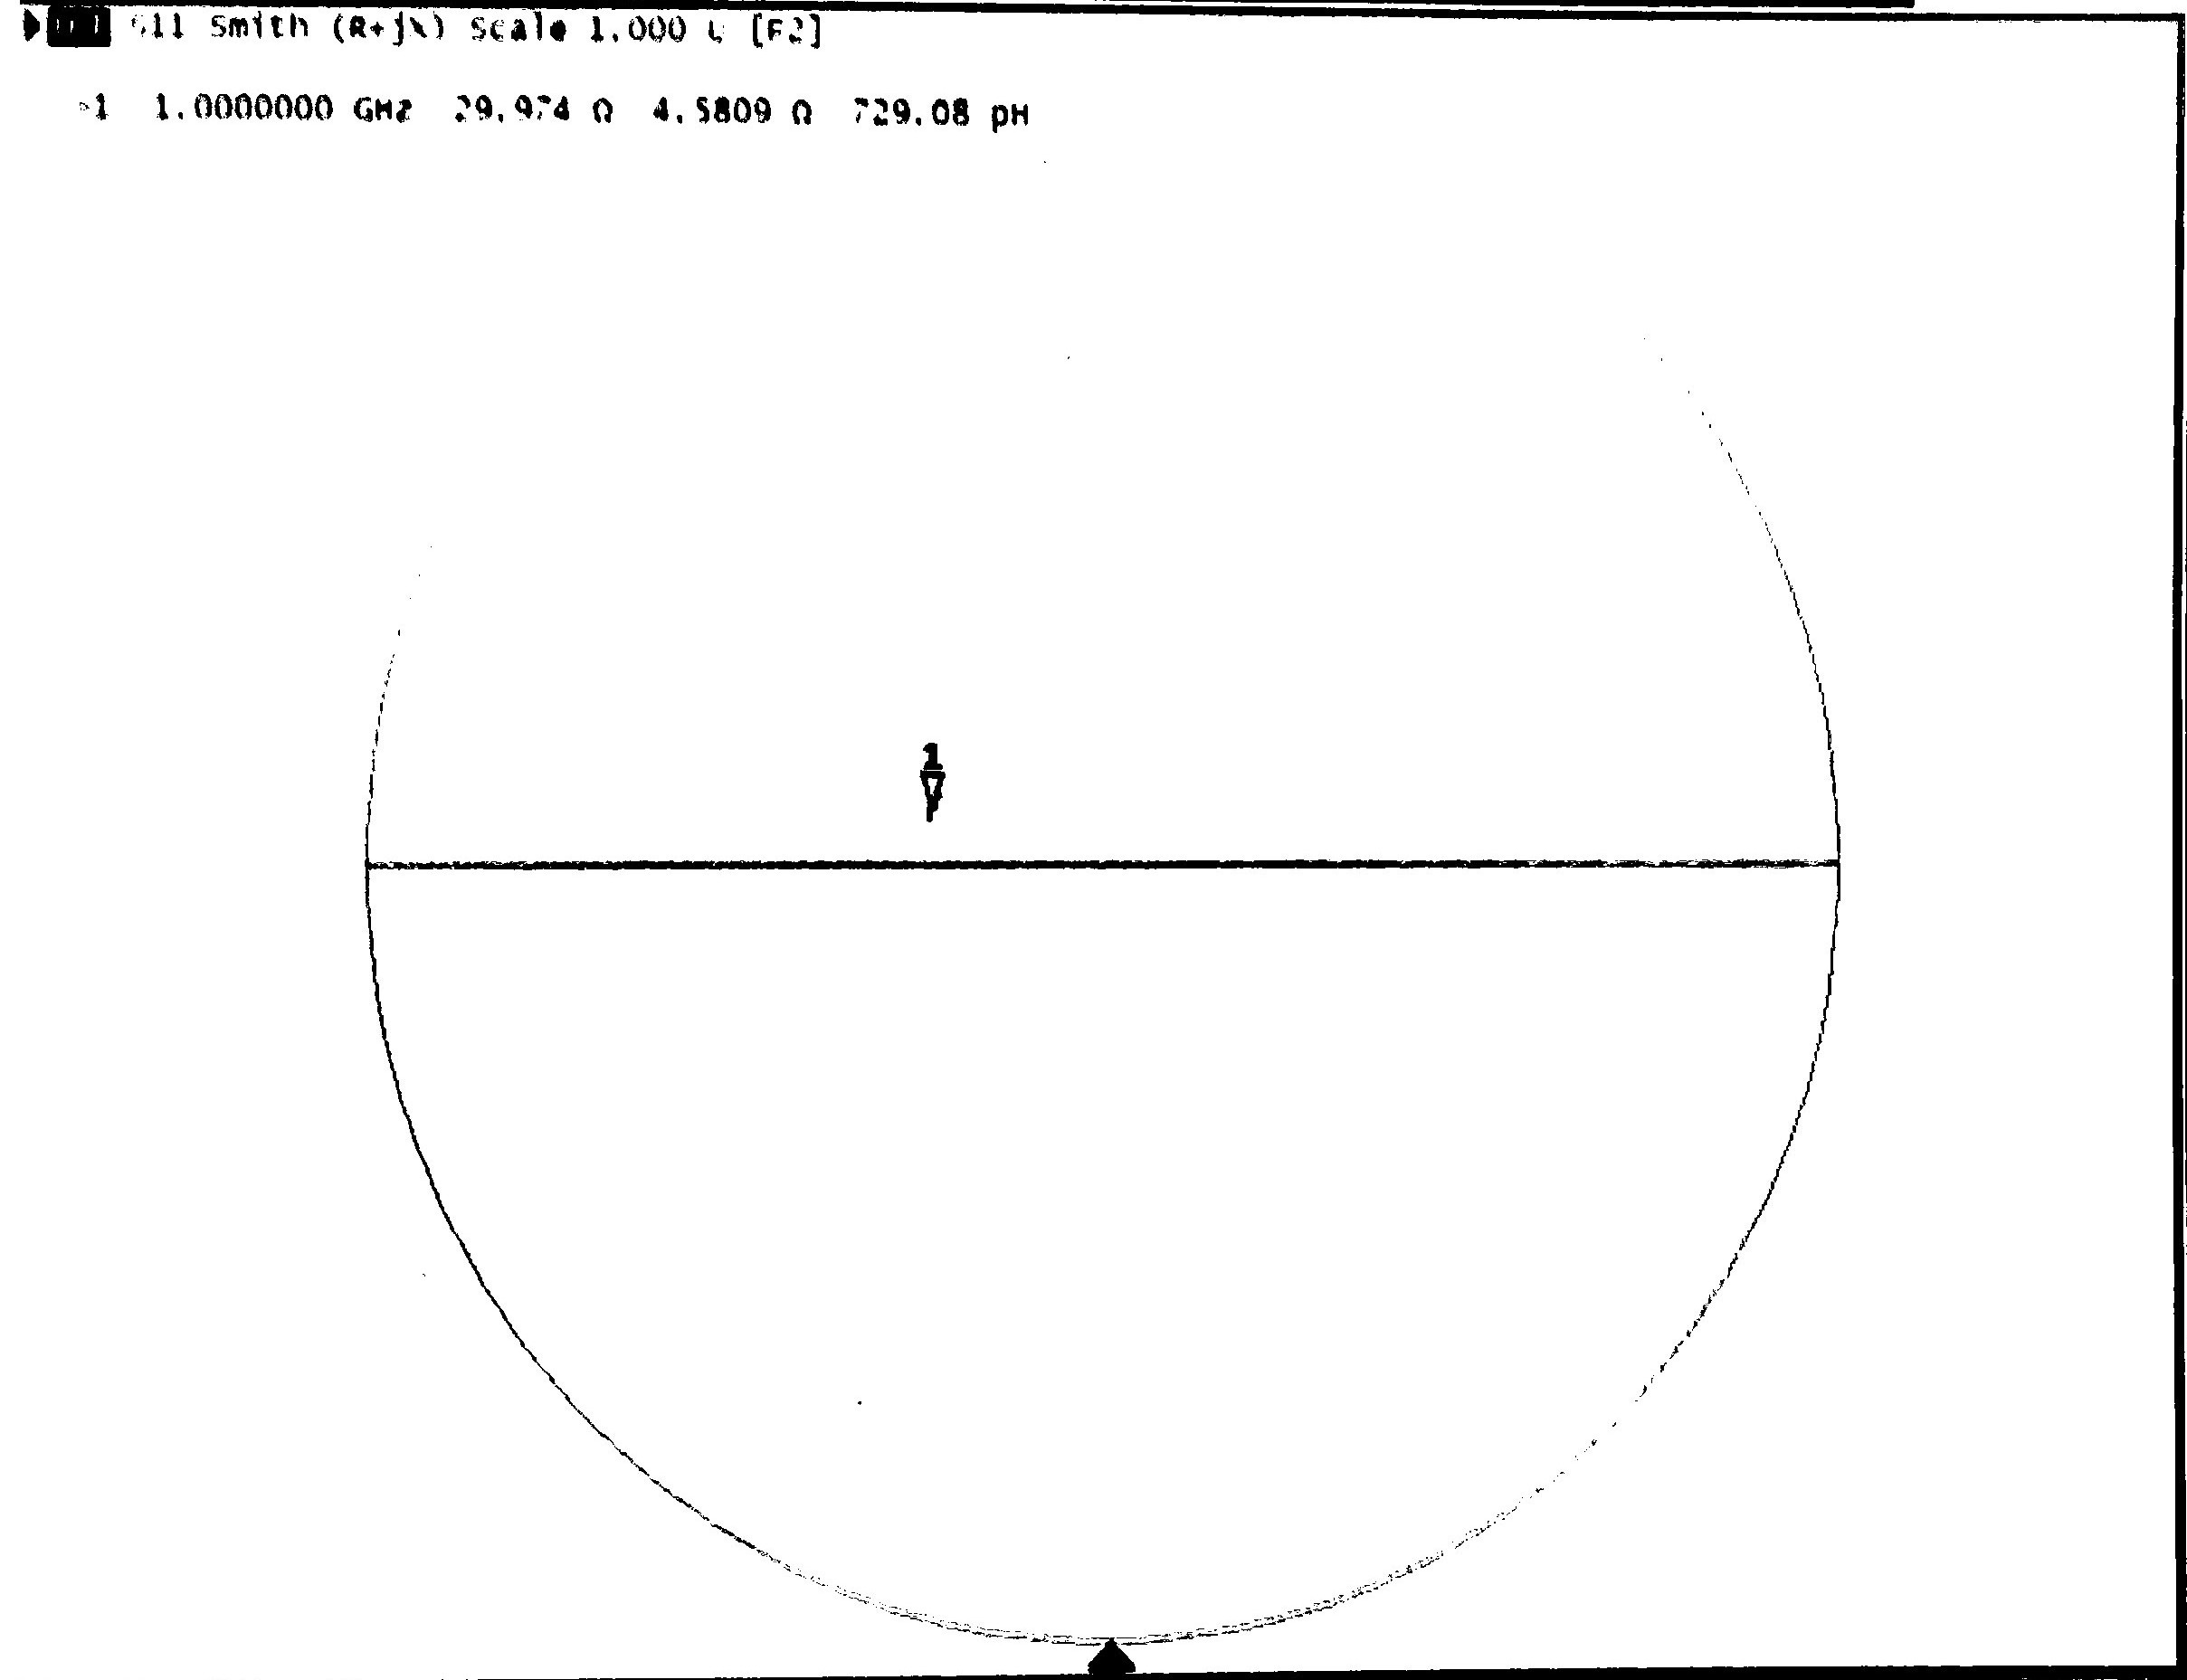
\includegraphics[width=0.45\textwidth]{../photos/lab2/unkwn-load.jpg}
    \caption{Transmission line terminated with load $Z_L = Z_0$\vspace{-0.5cm}}
    \label{tline_matching_z_0}
\end{figure}

% \section[Determining Z0 using V/I]{Determining $Z_0$ using $\frac{\tilde V^+(z=-L)}{\tilde I^+(z=-L)}$}

% \begin{figure}[ht] \centering
%     \begin{circuitikz} 
%         \draw
%         (0,2) to [sqV, l_=$\tilde V_g$] (0, 0) -- (2,0)
%         to [tline, l_=Transmission Line, o-o] (7,0)
%         to [R, l=$Z_L$] (7, 2)
%         to [tline, l=${Z_0, \beta, L}$, o-o] (2,2)
%         to [R, l_=$Z_g$, i<^=$\tilde I$] (0, 2);
        
%         \draw (2,2.35) node{$\tilde V$} (2, 2);
%         \draw (2,0) -- (2.5,-0.15) to[sV, l_=\footnotesize{CH1}, color=white, name=CH1] (2.5,1.75) -- (2, 2);
%         \oscope{CH1}{0}
%         \draw (7,0) -- (8,-0.15) to[sV, l_=\footnotesize{CH2}, color=white, name=CH2] (8,1.75) -- (7, 2);
%         \oscope{CH2}{0}
%         \draw (0,0) to[short, *-*] node[ground]{} (0,0);
%         \draw [dotted] (2,-0.35) -- (2,0.35) (7,-0.35) -- (7,0.35)
%         (2.1, -0.5) node{$z=-L$} (2, -0.35) (7, -0.5) node{$z=0$} (7, -0.35);
%     \end{circuitikz}
%     \caption{Laborartory setup for studying characteristcs of tranmission lines\vspace{-0.5cm}}
%     \label{tline_diag}
% \end{figure}

% \begin{figure}[ht]
%     \centering
%     \begin{subfigure}[b]{0.45\textwidth}
%         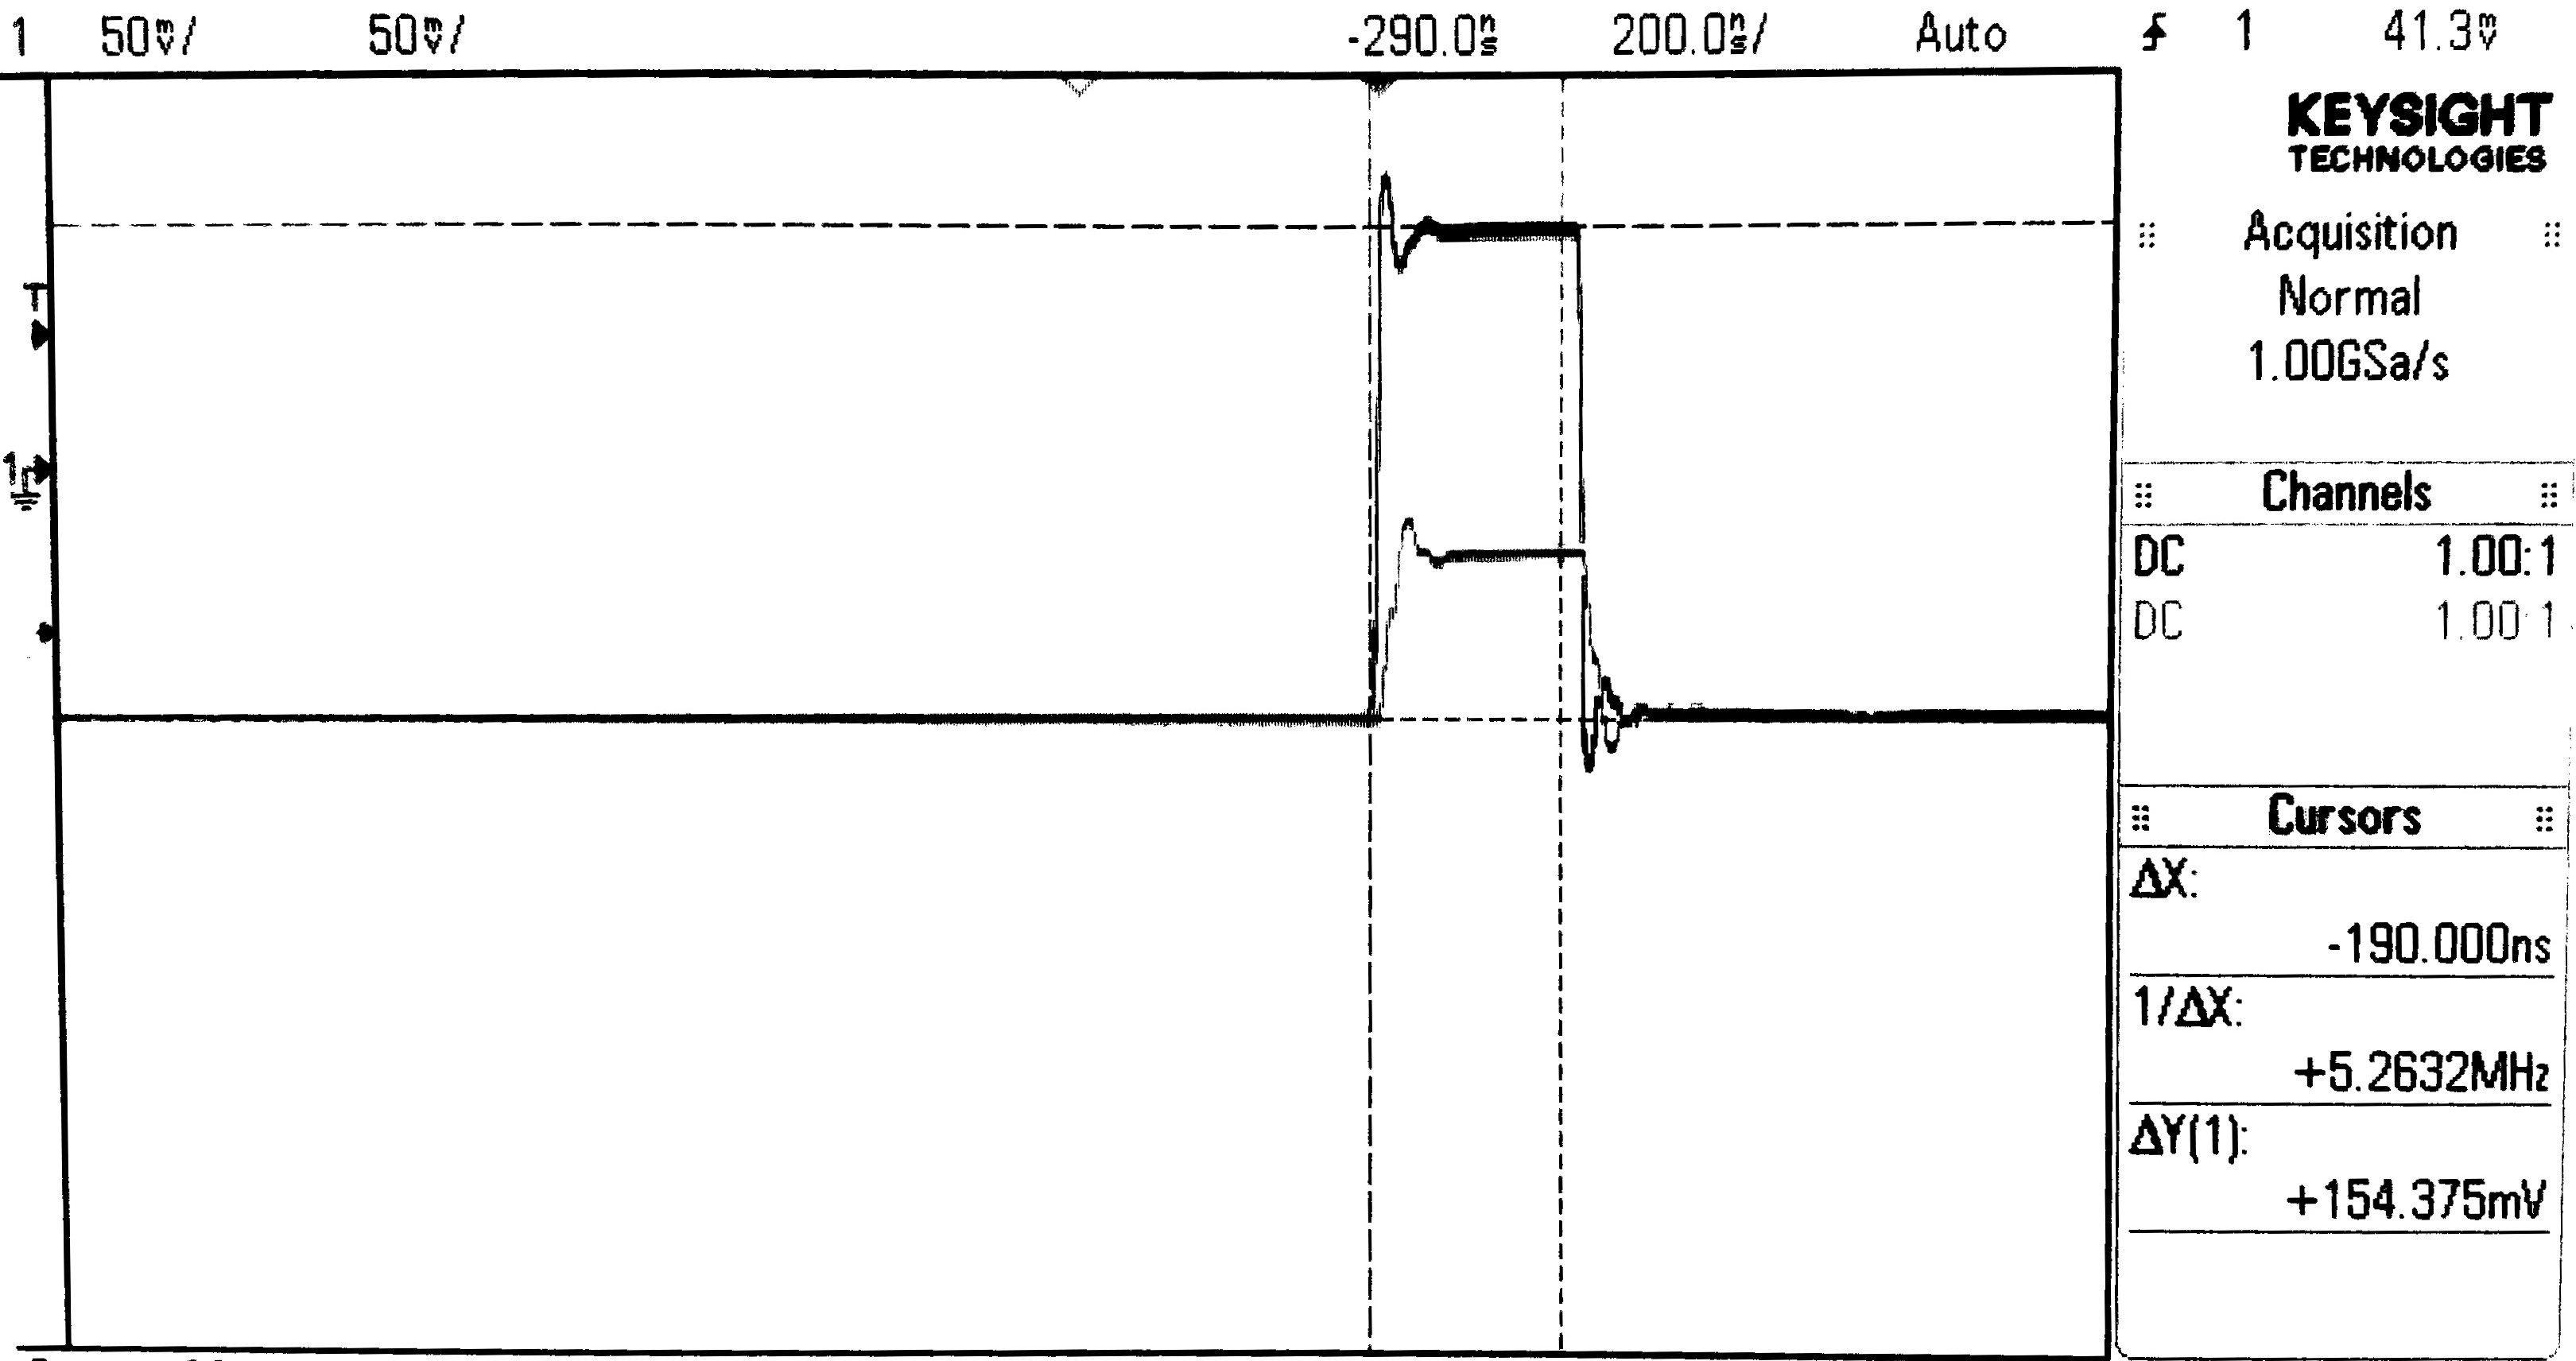
\includegraphics[width=\textwidth]{../photos/lab1/shunt_delta_v_1.jpg}
%         \caption{$\tilde V_1 \approx 154\text{mV}$}
%     \end{subfigure}
%     \quad
%     \begin{subfigure}[b]{0.45\textwidth}
%         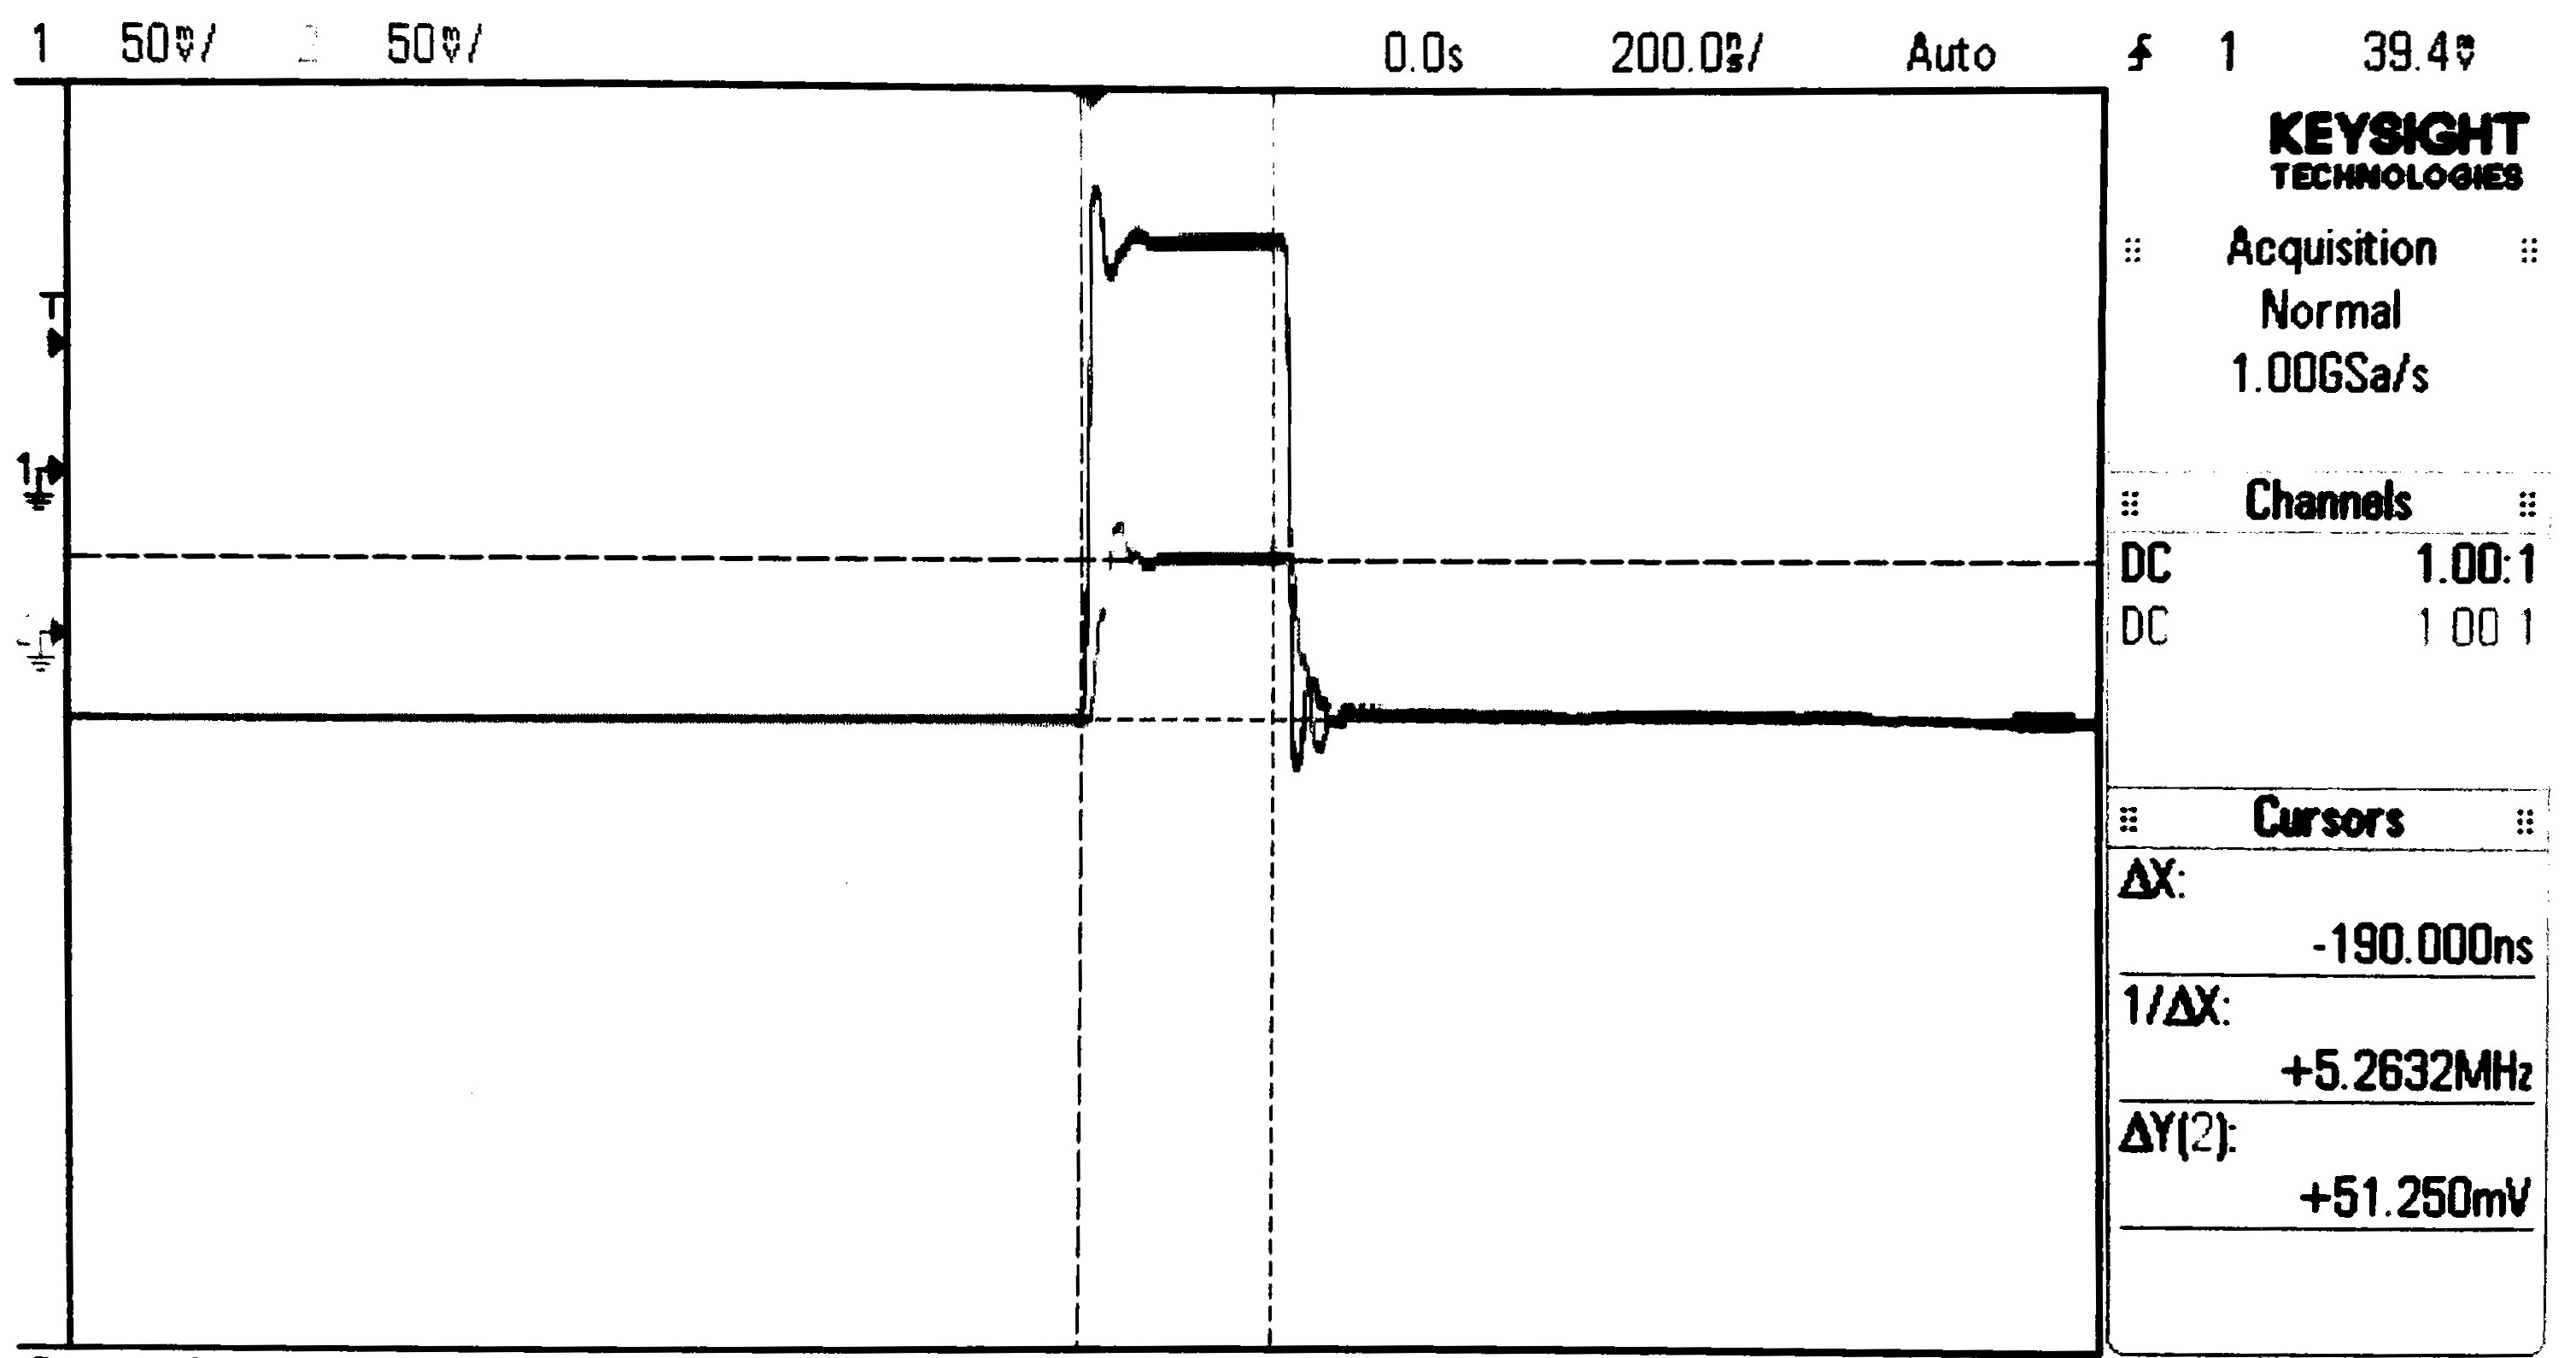
\includegraphics[width=\textwidth]{../photos/lab1/shunt_delta_v_2.jpg}
%         \caption{$\tilde V_2 \approx 51\text{mV}$}
%     \end{subfigure}
%     \caption{$\tilde V$ measured across $R_\text{shunt} = 100\Omega$\vspace{-0.5cm}}
%     \label{delta_v_shunt}
% \end{figure}

% As seen in Figure 3, the voltage at $\tilde V_1 = 154\text{mV}$ and $\tilde V_2 = 51\text{mV}$. Given the value of $R_\text{shunt} = 100\Omega$,
% we can calculate $\tilde I^+ = \frac{0.154-0.051}{100} = 1.03\text{mA}$. From Figure 4, we can see that $\tilde V_2 = \tilde V^+$, and therefore we can confirm the
% value of $Z_0$ through the relation, $Z_0 := \frac{\tilde V^+(z=-L)}{\tilde I^+(z=-L)} = \frac{51\text{mV}}{1.03\text{mA}} = 49.51\Omega \approx 50\Omega$.

% \begin{figure}[h] \centering
%     \begin{circuitikz} 
%         \draw [dotted][thick] (0,0) -- (0,2) (2,0) -- (2,2) (0, 2) -- (-1, 2) (2, 2) -- (3, 2);
%         \draw (0,1.5) to [R, l=$R_{\text{shunt}}$, i>^=$\tilde I$, *-*] (2, 1.5);
%         \draw (0,0.15) -- (2, 0.15);
%         \draw (1, 0.15) to [short, *-*] node[ground]{} (1,0.15);
%         \draw (0,0.15) circle (1.5pt);
%         \draw (2,0.15) circle (1.5pt);
%         \draw (2,0.15) -- (2.5,-0.15) to[sV, l_=$\tilde V_2$, color=white, name=CH2] (2.5,1.35) -- (2, 1.5);
%         \oscope{CH2}{0}
%         \draw (0,0.15) -- (-0.5,-0.15) to[sV, l=$\tilde V_1$, color=white, name=CH1] (-0.5,1.35) -- (0, 1.5);
%         \oscope{CH1}{0}

%         \draw (4.75,1) node[]{$\displaystyle{\tilde I = \frac{\tilde V_1 - \tilde V_2}{R_{\text{shunt}}}}$} (4.75,1);
%     \end{circuitikz}
%     \caption{Estimating input current through a shunt resistance \vspace{-0.5cm}}
%     \label{shunt_diag}
% \end{figure}

\section{Using Standing Wave Patterns for Load Calculations}

Observed waveforms at different points on the transmission line can be found in Figure 5.

\begin{figure}[ht]
    \centering
    \begin{subfigure}[b]{0.45\textwidth}
        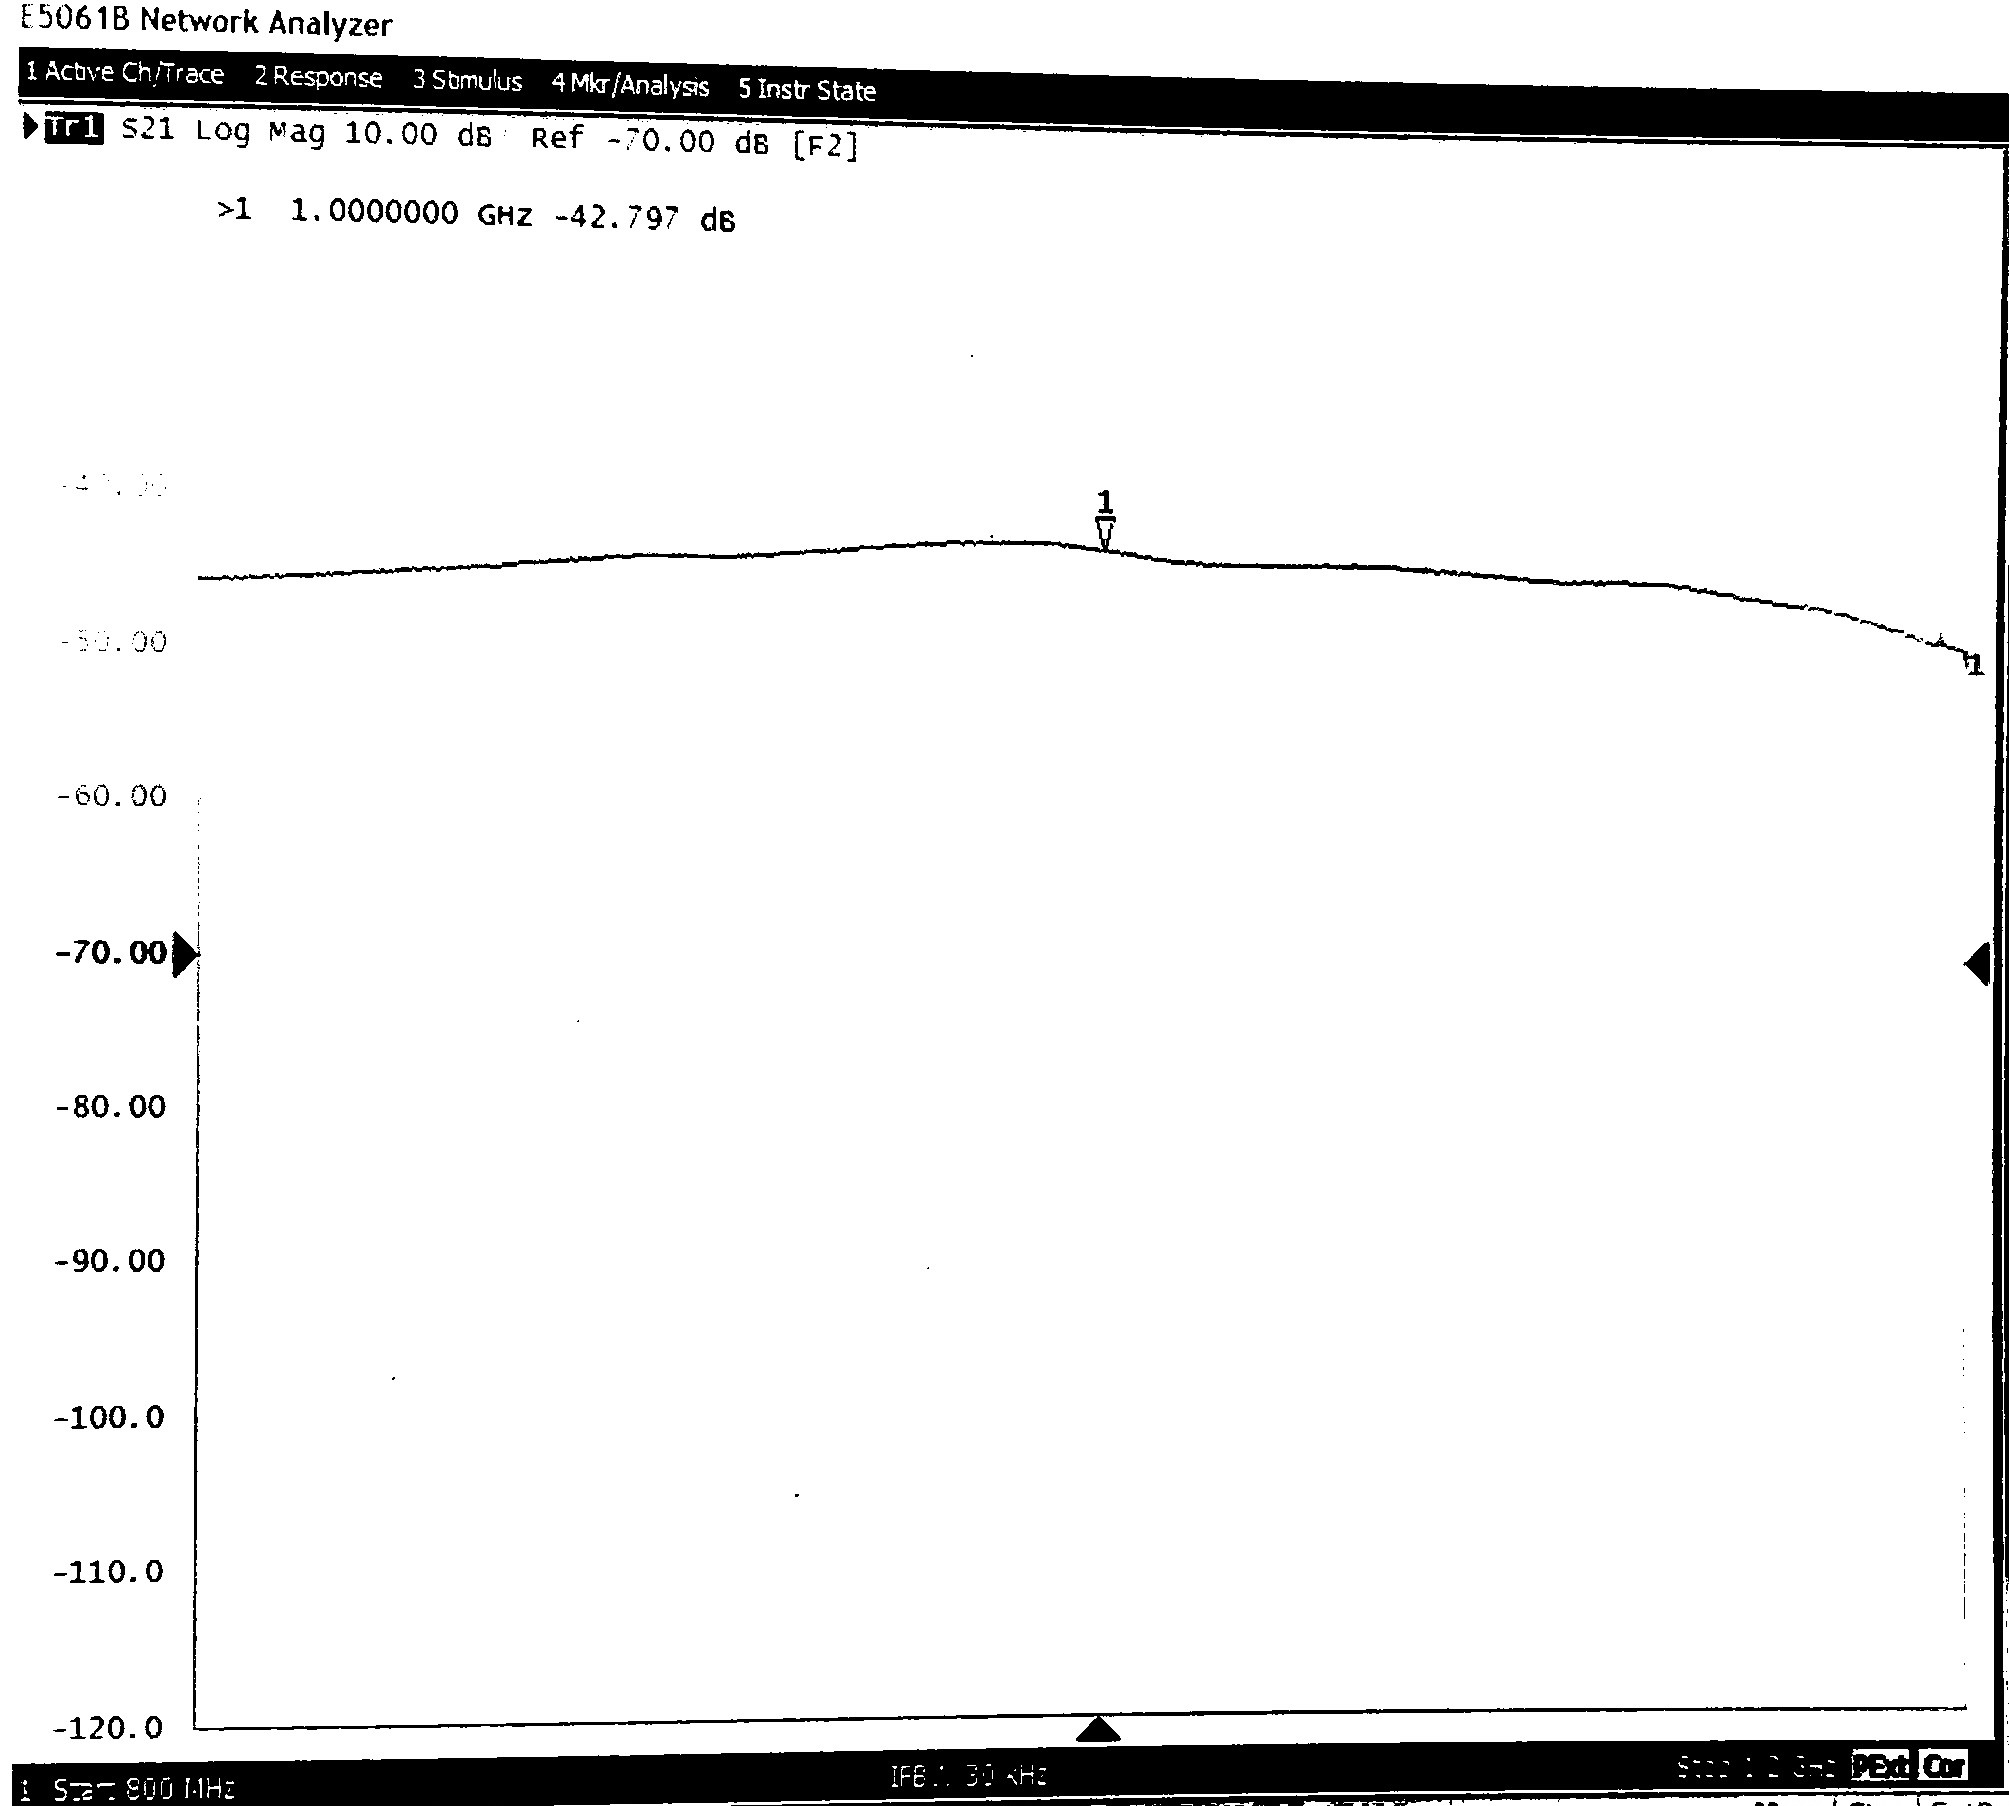
\includegraphics[width=\textwidth]{../photos/lab2/short-cir-peak.jpg}
        \caption{Port C $(0\text{m})$}
    \end{subfigure}
    \quad
    \begin{subfigure}[b]{0.45\textwidth}
        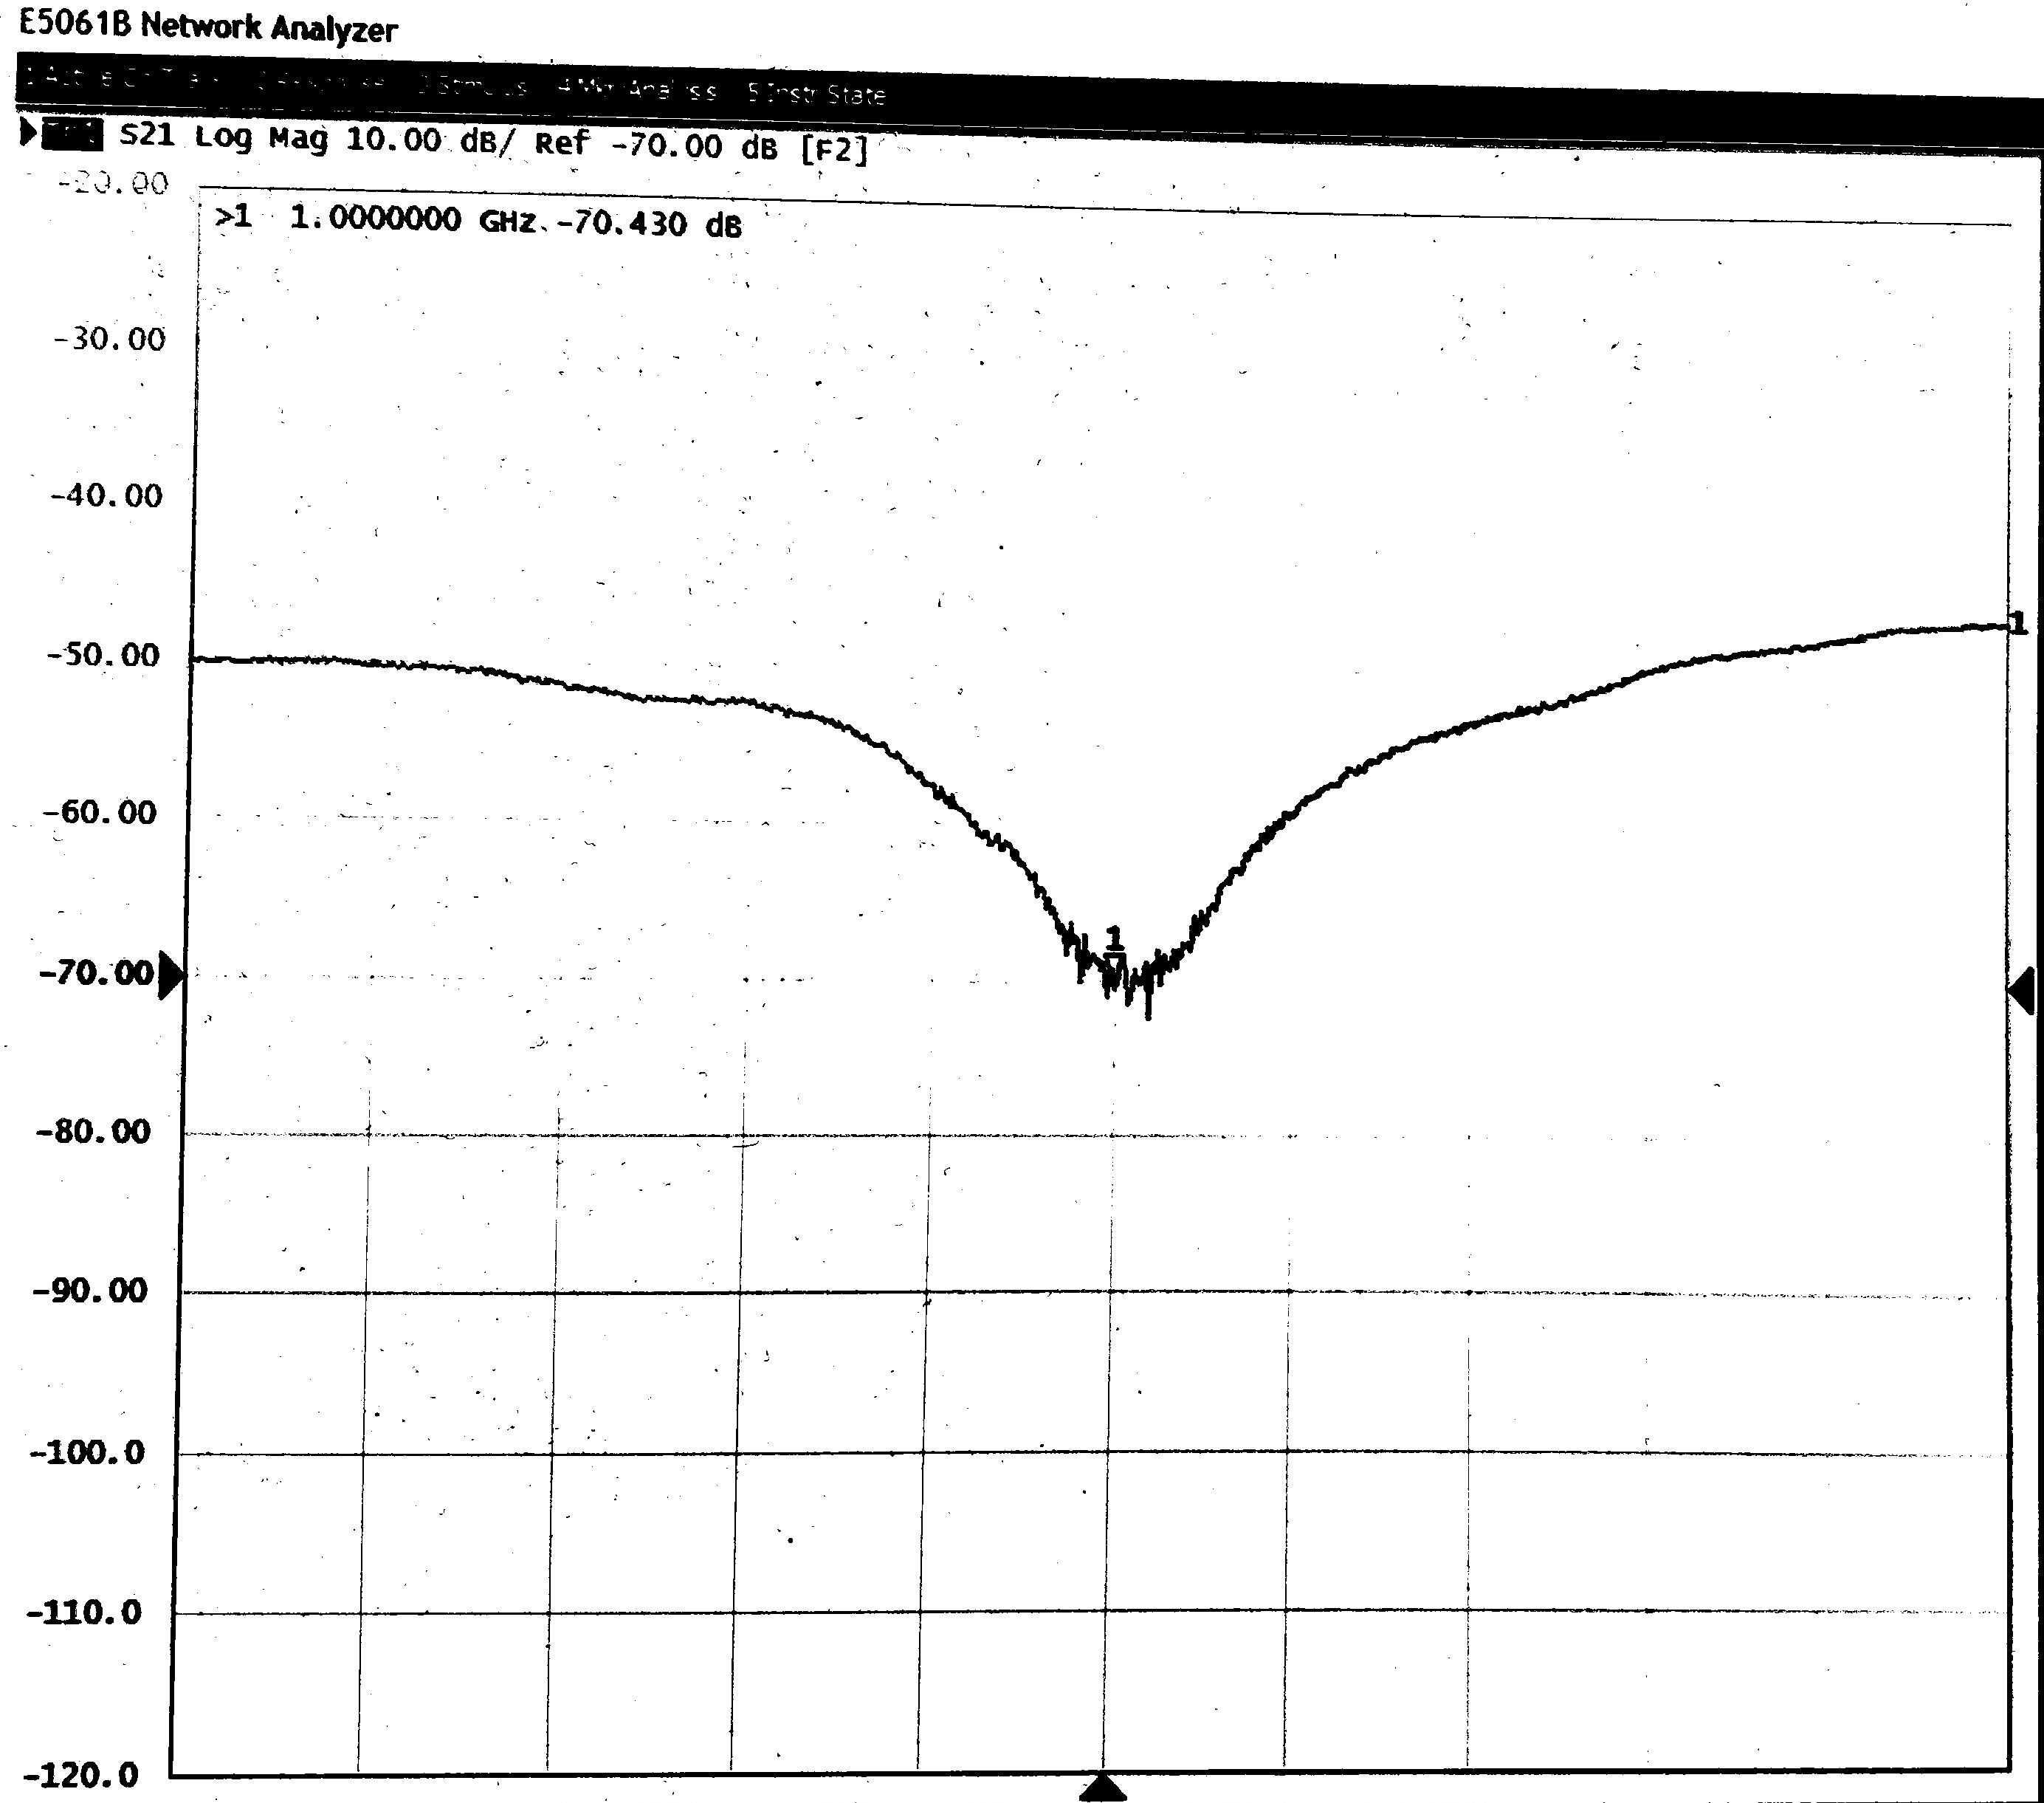
\includegraphics[width=\textwidth]{../photos/lab2/short-cir-valley.jpg}
        \caption{Port D $(30\text{m})$}
    \end{subfigure}
    \begin{subfigure}[b]{0.45\textwidth}
        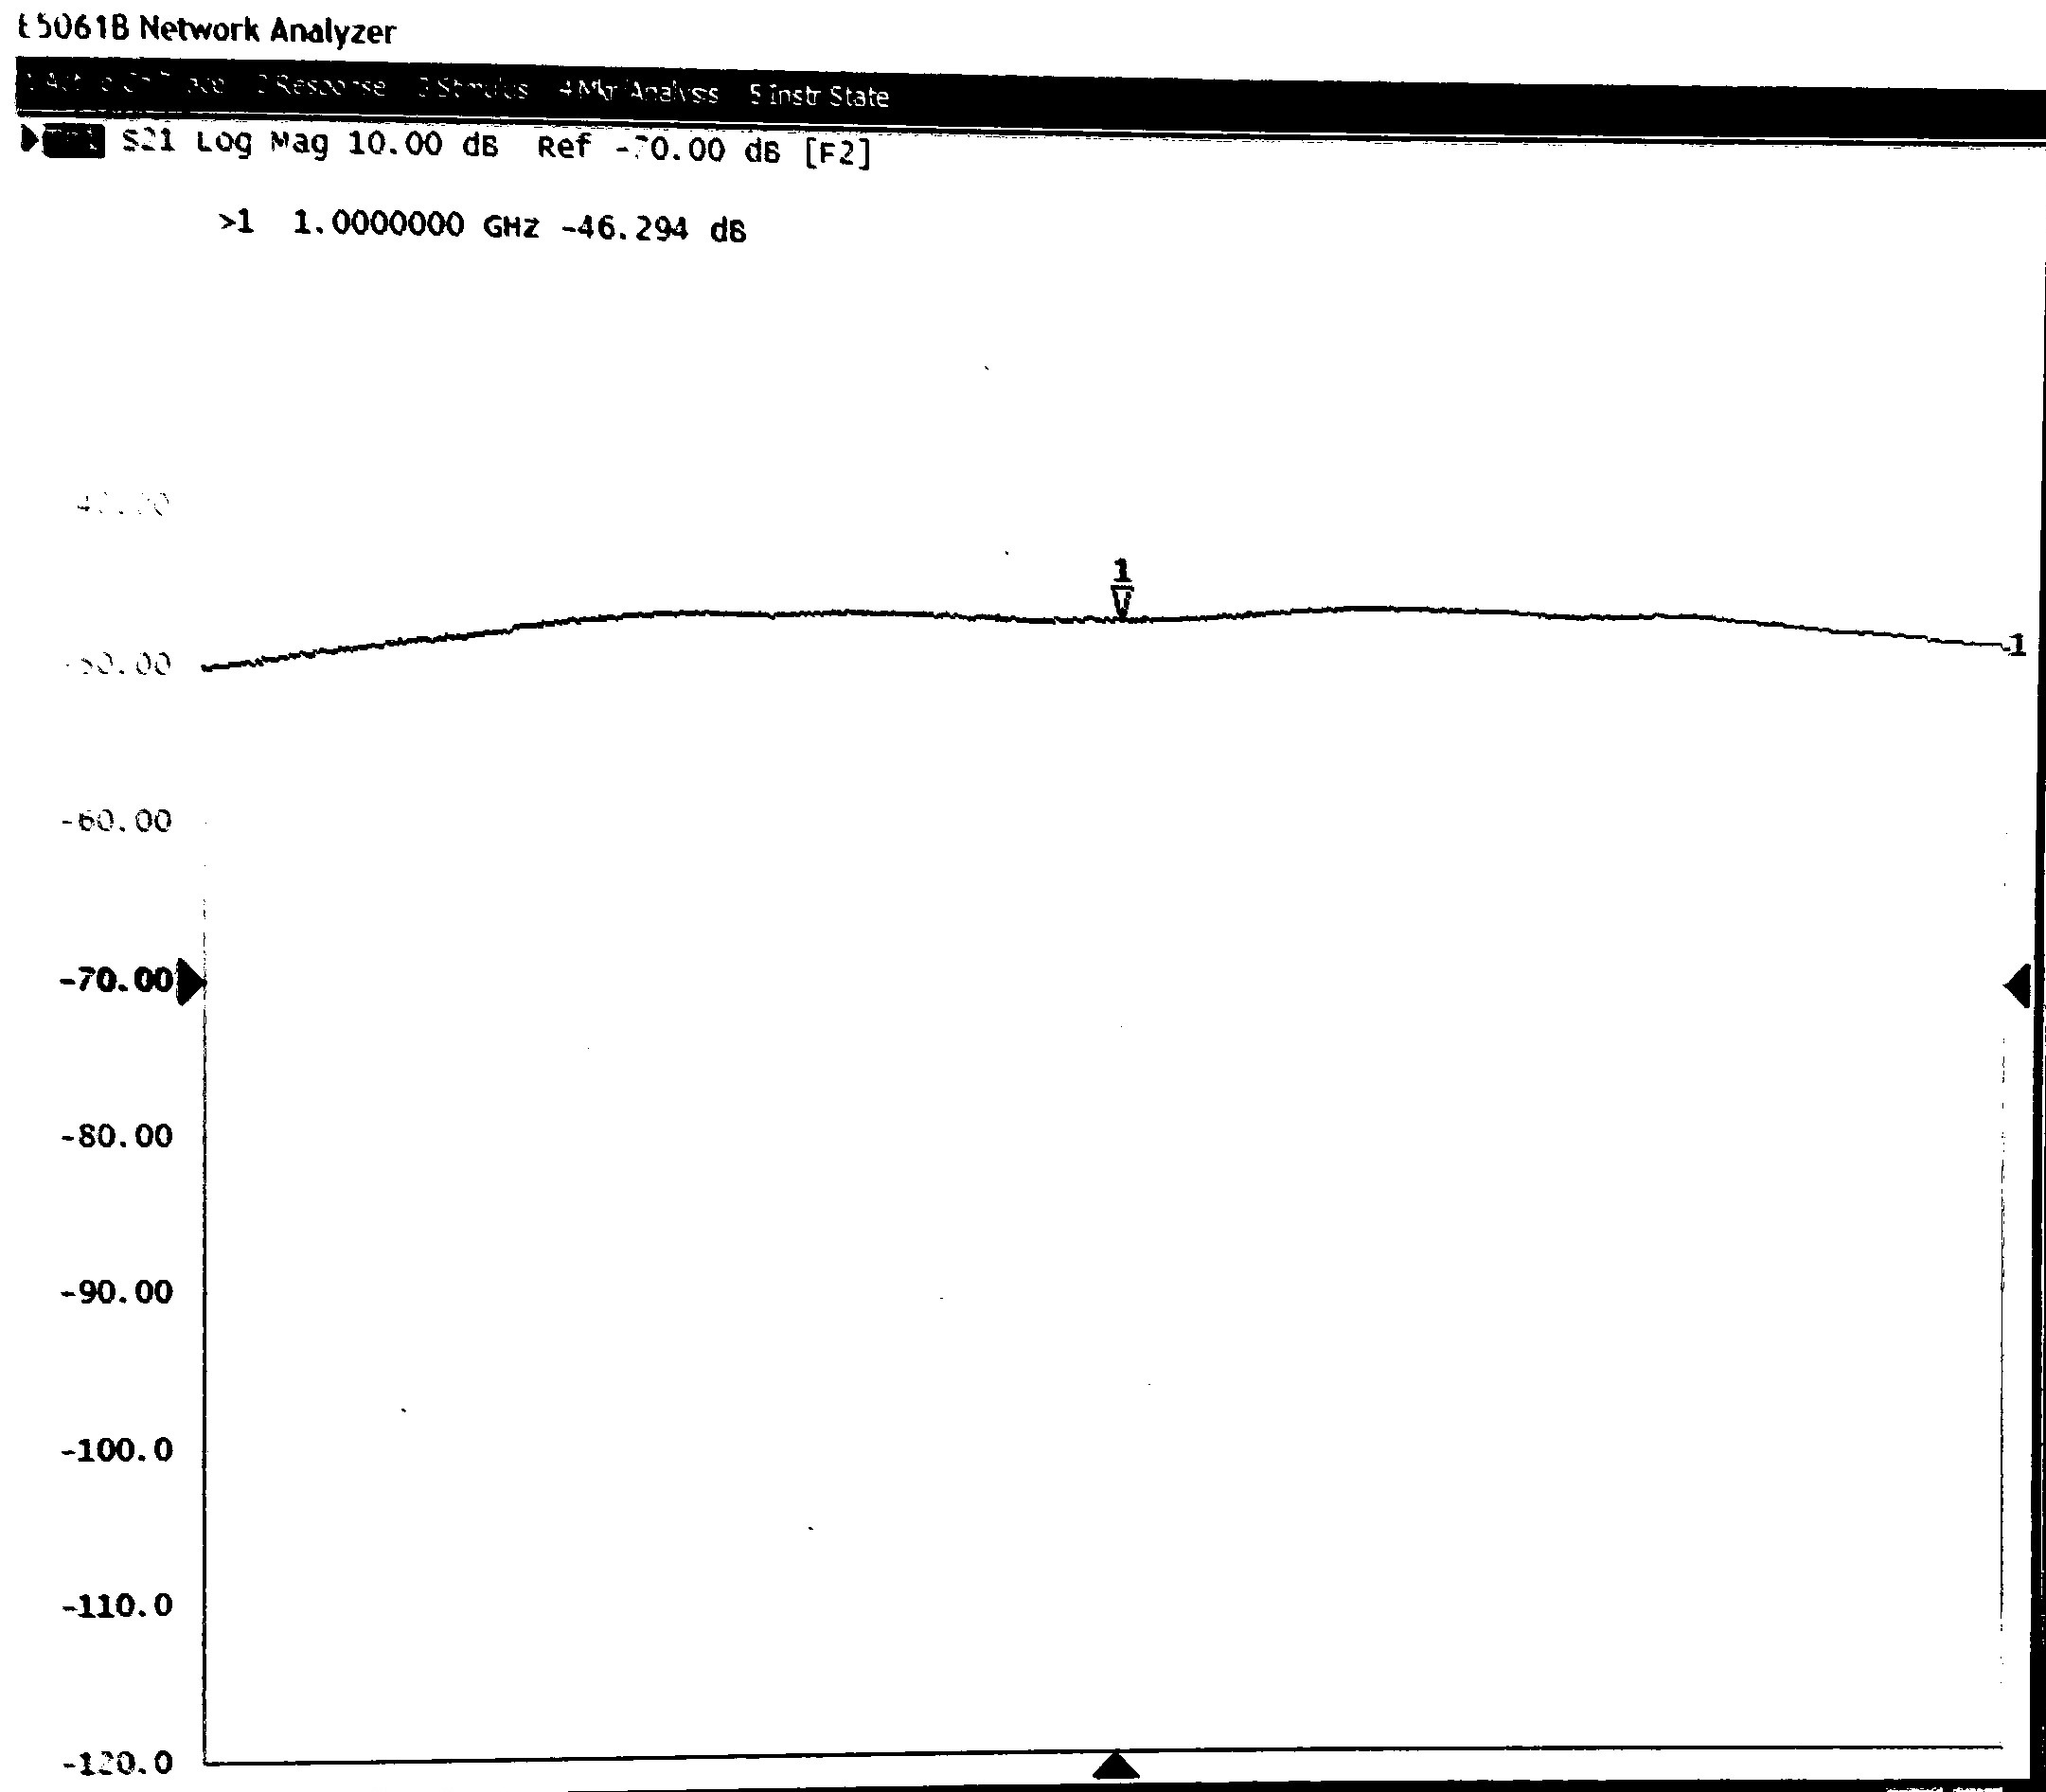
\includegraphics[width=\textwidth]{../photos/lab2/unkwn-load-peak.jpg}
        \caption{Port E $(60\text{m})$}
    \end{subfigure}
    \quad
    \begin{subfigure}[b]{0.45\textwidth}
        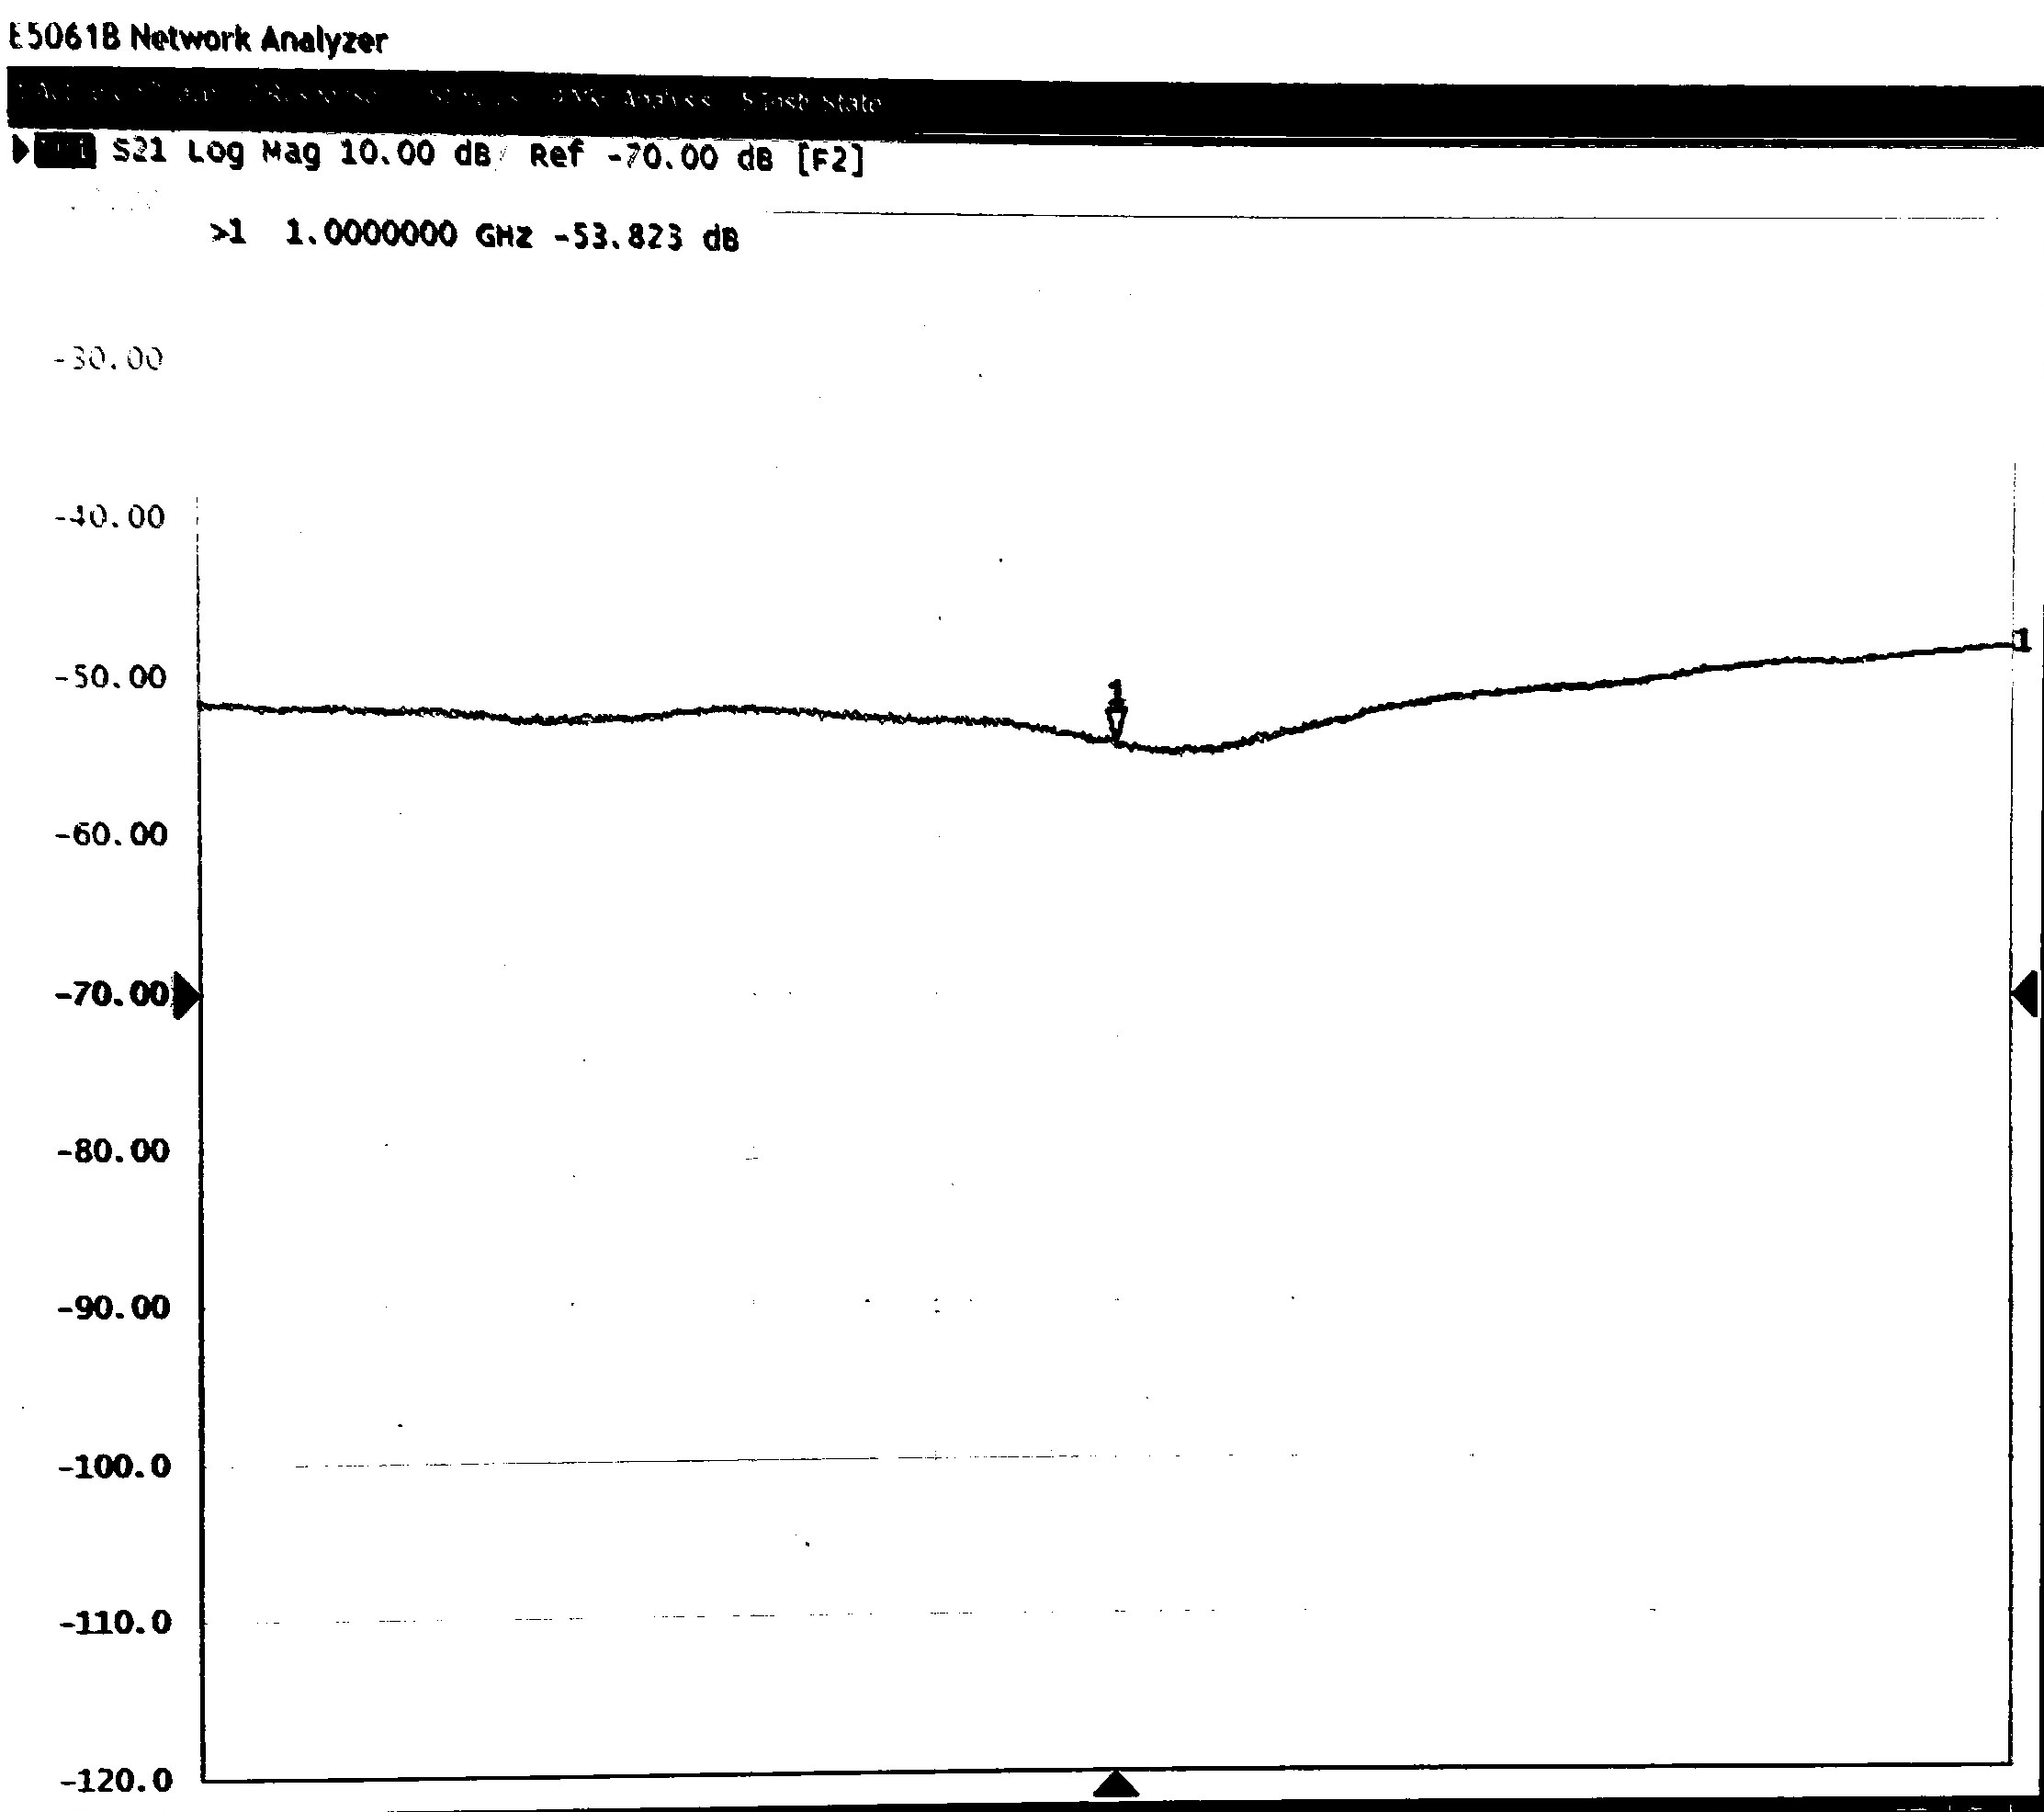
\includegraphics[width=\textwidth]{../photos/lab2/unkwn-load-valley.jpg}
        \caption{Port F $(90\text{m})$}
    \end{subfigure}
    \caption{Measured $V(t)$ at different loactions along the transmission line with $Z_L = Z_0$ \vspace{-0.5cm}}
    \label{v_t_matched_tline}
\end{figure}

% The recorded time delays, $\Delta t$, relative to the input signal are listed in Table 1.

% \begin{table}[h]
%     \[
%         \begin{array}{c|c}
%             \textbf{Port} & \Delta t \textbf{ (ns)} \\ \hline
%             \text{D} & 130\\
%             \text{E} & 244\\
%             \text{F} & 368
%         \end{array}
%     \]
%     \caption{Recorded time delay at different locations along the transmission line\vspace{-0.5cm}}
% \end{table}

% \section{Determining Velocity of Propagation}

% The velocity of propagation of the signal can be calculated by the relation $v_p = \frac{\Delta L}{\Delta t}$, given that
% we are able to track the same point on the waveform. Using the data from Table 1,
% we get that the average velocity of propagation is $v_{p, \text{avg}} = 2.44 \cdot 10^8 \text{m/s}$.

% Now, to find the relative permittivity, we also know that the phase velocity of an electromagentic wave in an electrical transmission line with magnetic permeability, $\mu \approx \mu_0$,
% and electric permittivity, $\epsilon = \epsilon_r \epsilon_0$,  is given by: 

% \[
%     v_p = \frac{1}{\sqrt{\mu \epsilon}} \implies \frac{v_p}{c} \approx 
%     \sqrt{\frac{\mu_0\epsilon_0}{\mu_0\epsilon_0\epsilon_r}} \implies 
%     \epsilon_r \approx \frac{c^2}{v_p^2} \approx 1.51
% \]

% The theoretical $V(t)$ plots in Figure 6 closely match the observations in Figure 5.

% \begin{figure}[h]
%     \centering
%     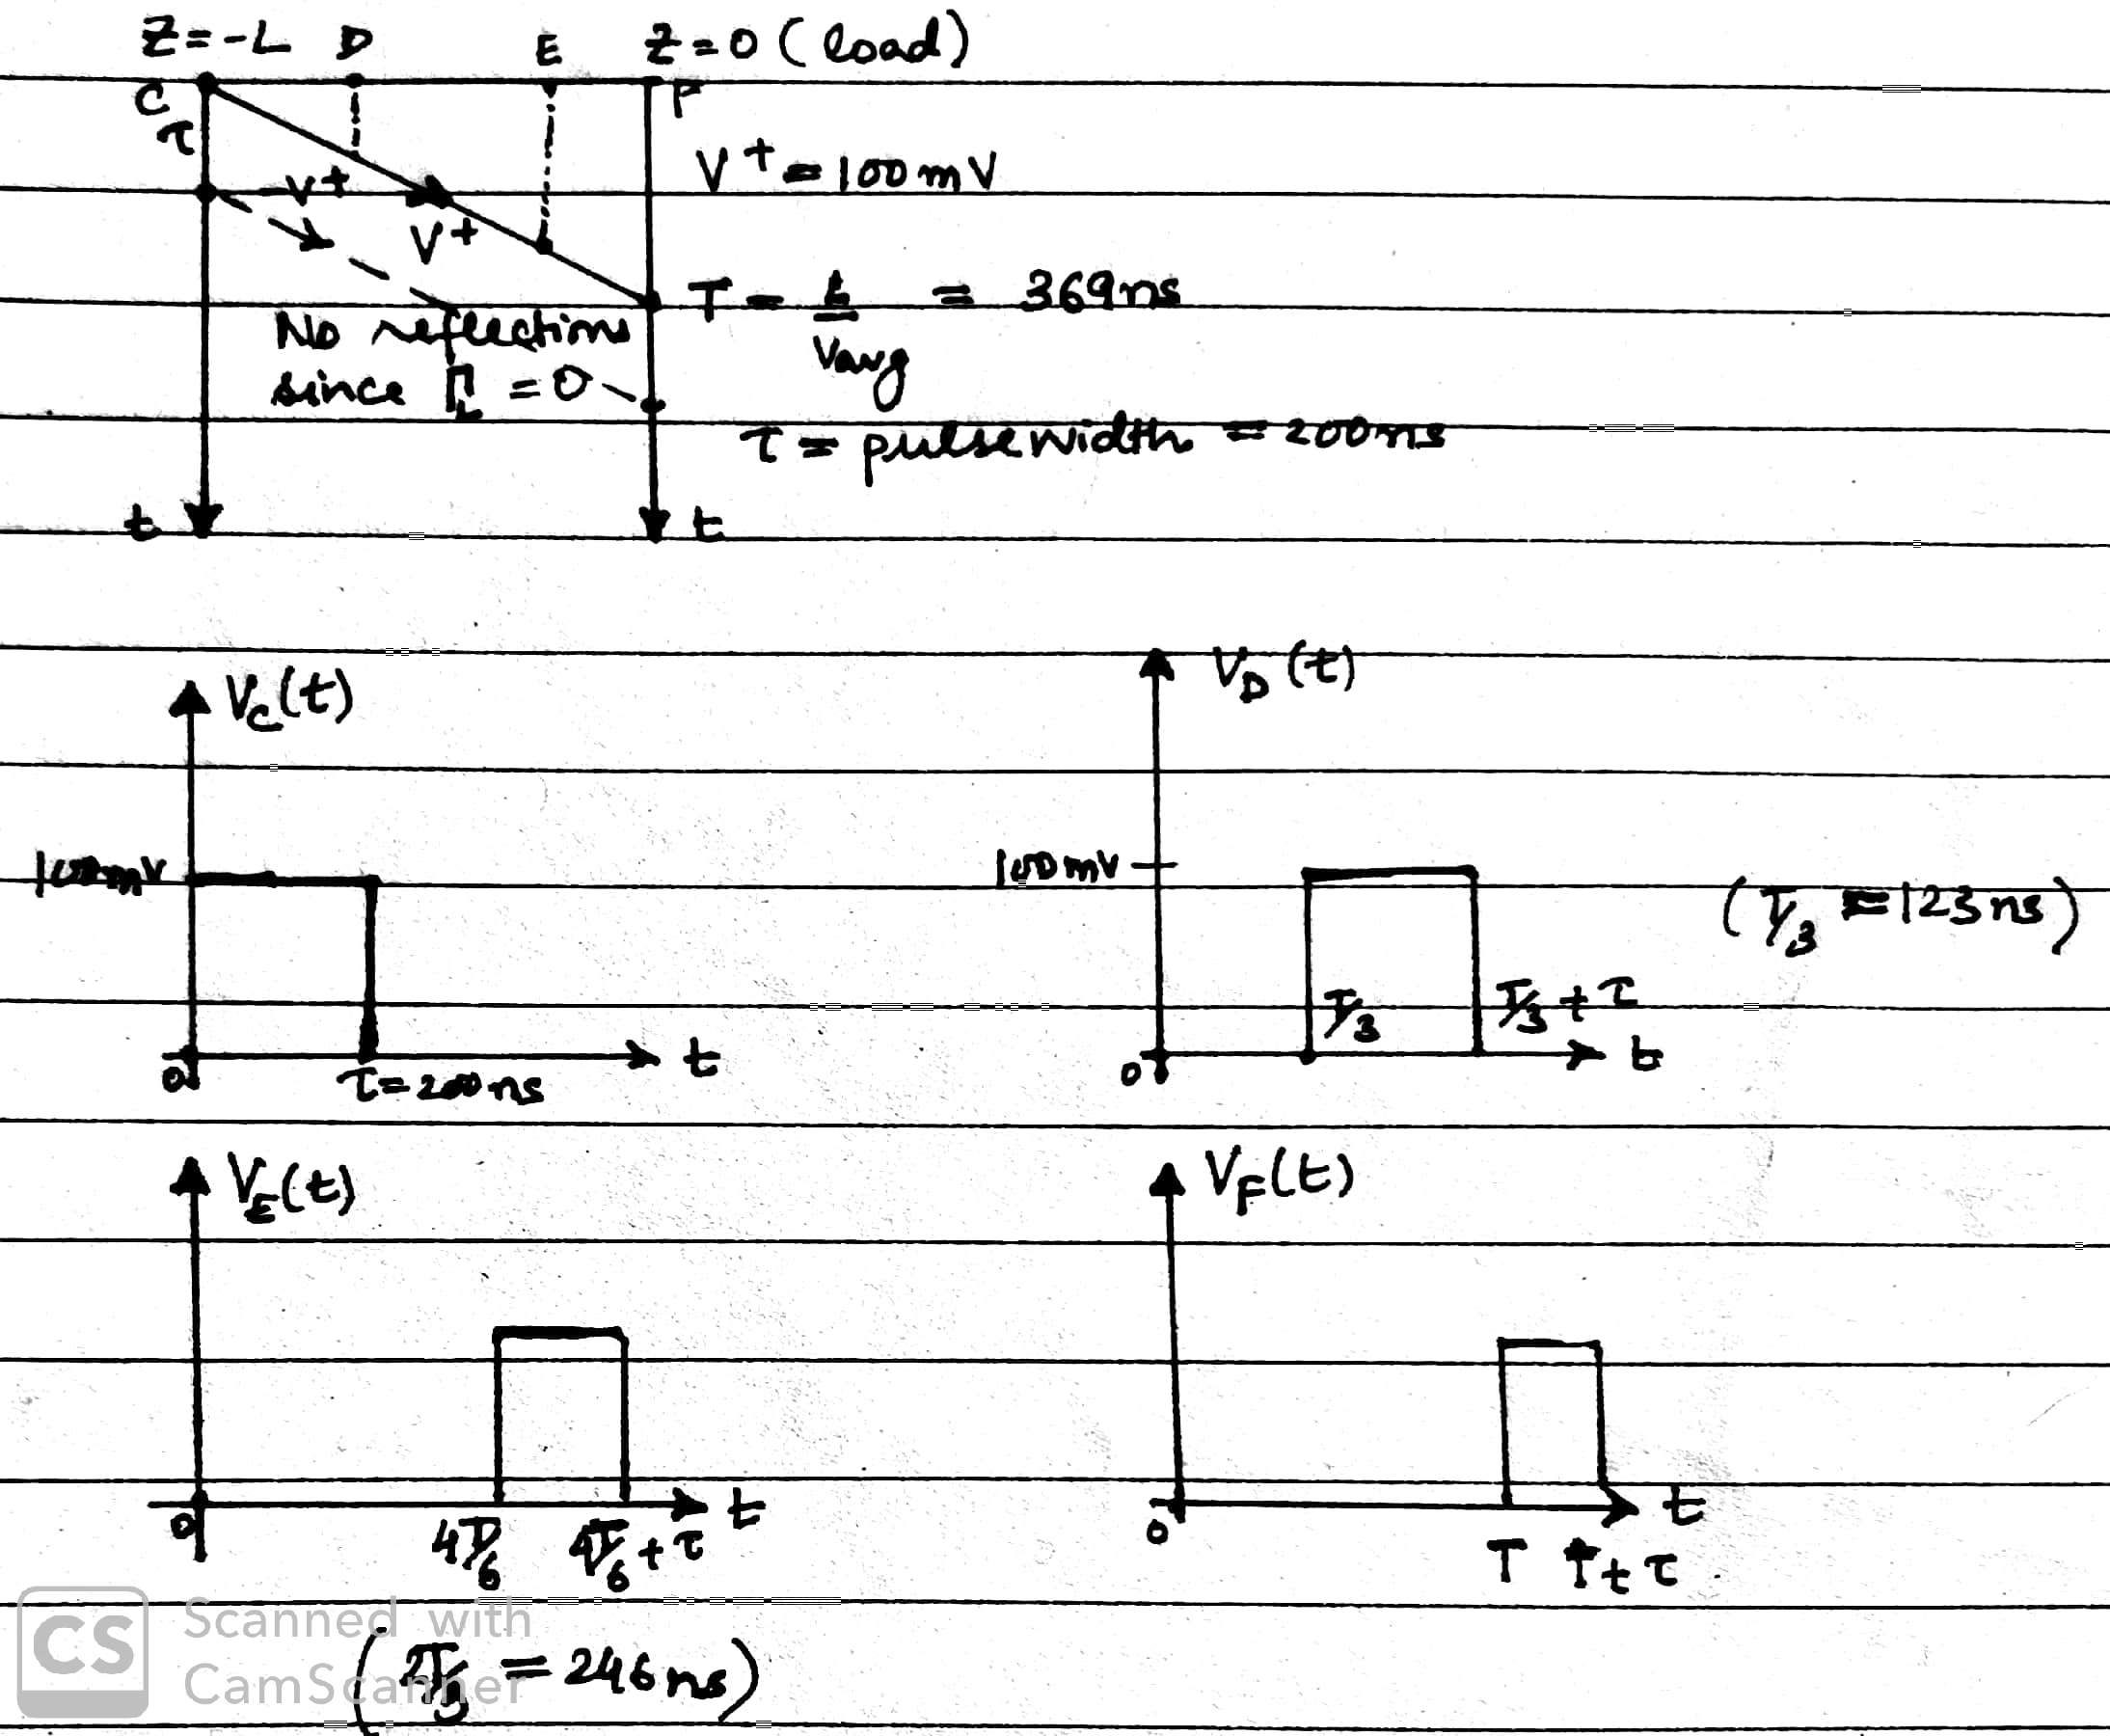
\includegraphics[width=0.45\textwidth]{../photos/lab1/v_t_bounce_no_reflection.jpg}
%     \caption{Theoretical bounce diagram and $V(t)$ plots along the transmission line\vspace{-0.5cm}}
%     \label{v_t_bounce_no_reflection}
% \end{figure}

% \section{Simple Reflection}

% For an input pulse signal, the magnitude of the first voltage pulse across the transmission line input will always be $\tilde V^+_1 = \tilde V_g\frac{Z_0}{Z_0+Z_g}$, regardless of $Z_L$. There will be a load mismatch if $Z_L \neq Z_0$ and we know that, in this case, reflection of current and
% voltage occurs at the load, i.e. $\tilde V^- \neq 0$ and $\tilde I^- \neq 0$. The load reflection coefficient, $\Gamma_L$,
% if defined as:
% \[
%     \Gamma_L := \frac{\tilde V^-}{\tilde V^+} = \frac{Z_L - Z_0}{Z_L + Z_0}
% \]

% Thus, in cases where there is a load mismatch, $\Gamma_L \neq 0$, there will be a relection of intensity $\tilde V^- = \Gamma_L\tilde{V^+}$ along the 
% transmission line towards the generator and the steady state for a step input will be achieved after the voltage and current 
% wave has travelled back and forth once, and this can also be verified using a bounce diagram. The Theoretically for $Z_L = 100\Omega$, $\Gamma_L = \frac{50\Omega}{150\Omega} = \frac{1}{3} $ and through the measurements, we observe the reflection 
% coefficient $\Gamma_L = \frac{30\text{mV}}{100\text{mV}} = \frac{3}{10} \approx \frac{1}{3}$.

% The measurements for reflected voltage waves can be found in Figure 7. Channel 1 (top) waveform has been 
% recorded at port C ($0\text{m}$) and channel 2 (bottom) waveform has been recorded at port F ($90\text{m}$).
% The pulsewidth $\tau$ of the signal was set such that it was equal to the time delay $T$ for a pulse to reach
% port F from port C, which made the signal recordings at port C and F exactly out of phase. In terms of magnitude, the
% signal at port F was a superposition of the incident and reflected wave $\tilde V_F = \tilde V^+ + \Gamma_L\tilde V^+$.
% Similarly at port C, the signal at $t \in (2T, 3T)$, $\tilde V_C = \Gamma_L\tilde V^+ = \tilde V^-$, which can all again
% be verified using a bounce diagram. The theoretical $V(d)$ graphs for different time points can be found in Figure 8.

% \begin{figure}[ht]
%     \centering
%     \begin{subfigure}[b]{0.45\textwidth}
%         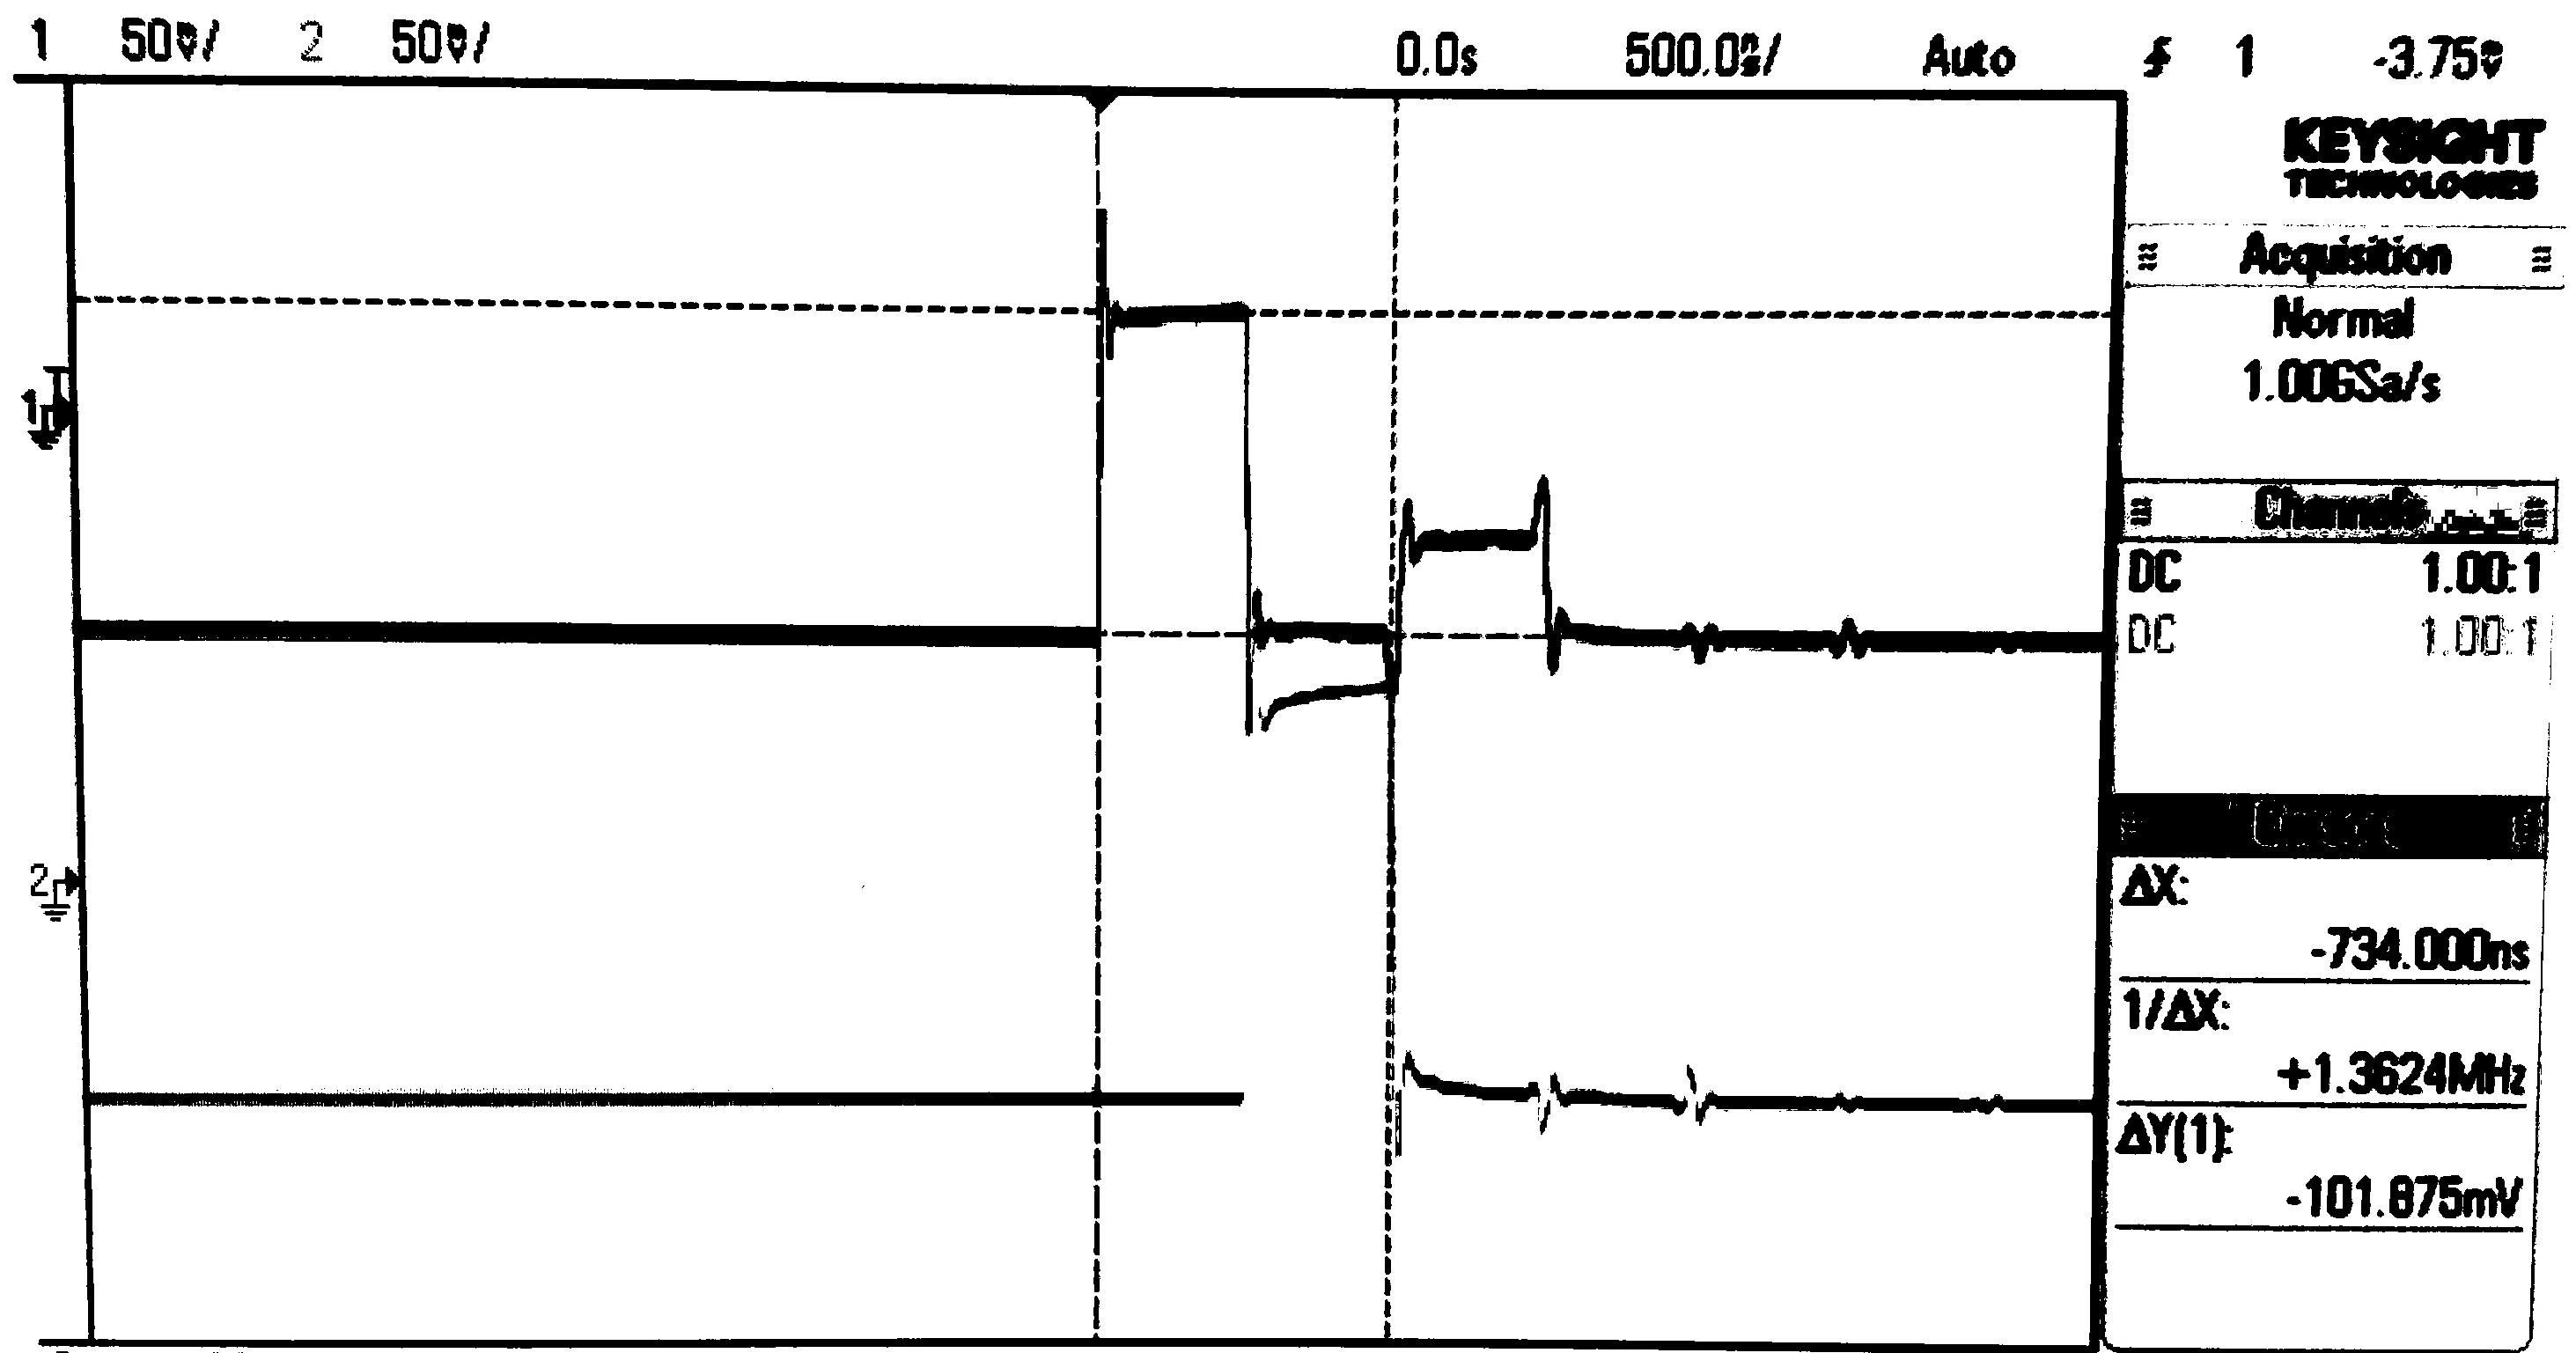
\includegraphics[width=\textwidth]{../photos/lab1/v_t_gamma_L_1.jpg}
%         \caption{$\tilde V_1 = \tilde V^+ \approx 100\text{mV}$}
%     \end{subfigure}
%     \quad
%     \begin{subfigure}[b]{0.45\textwidth}
%         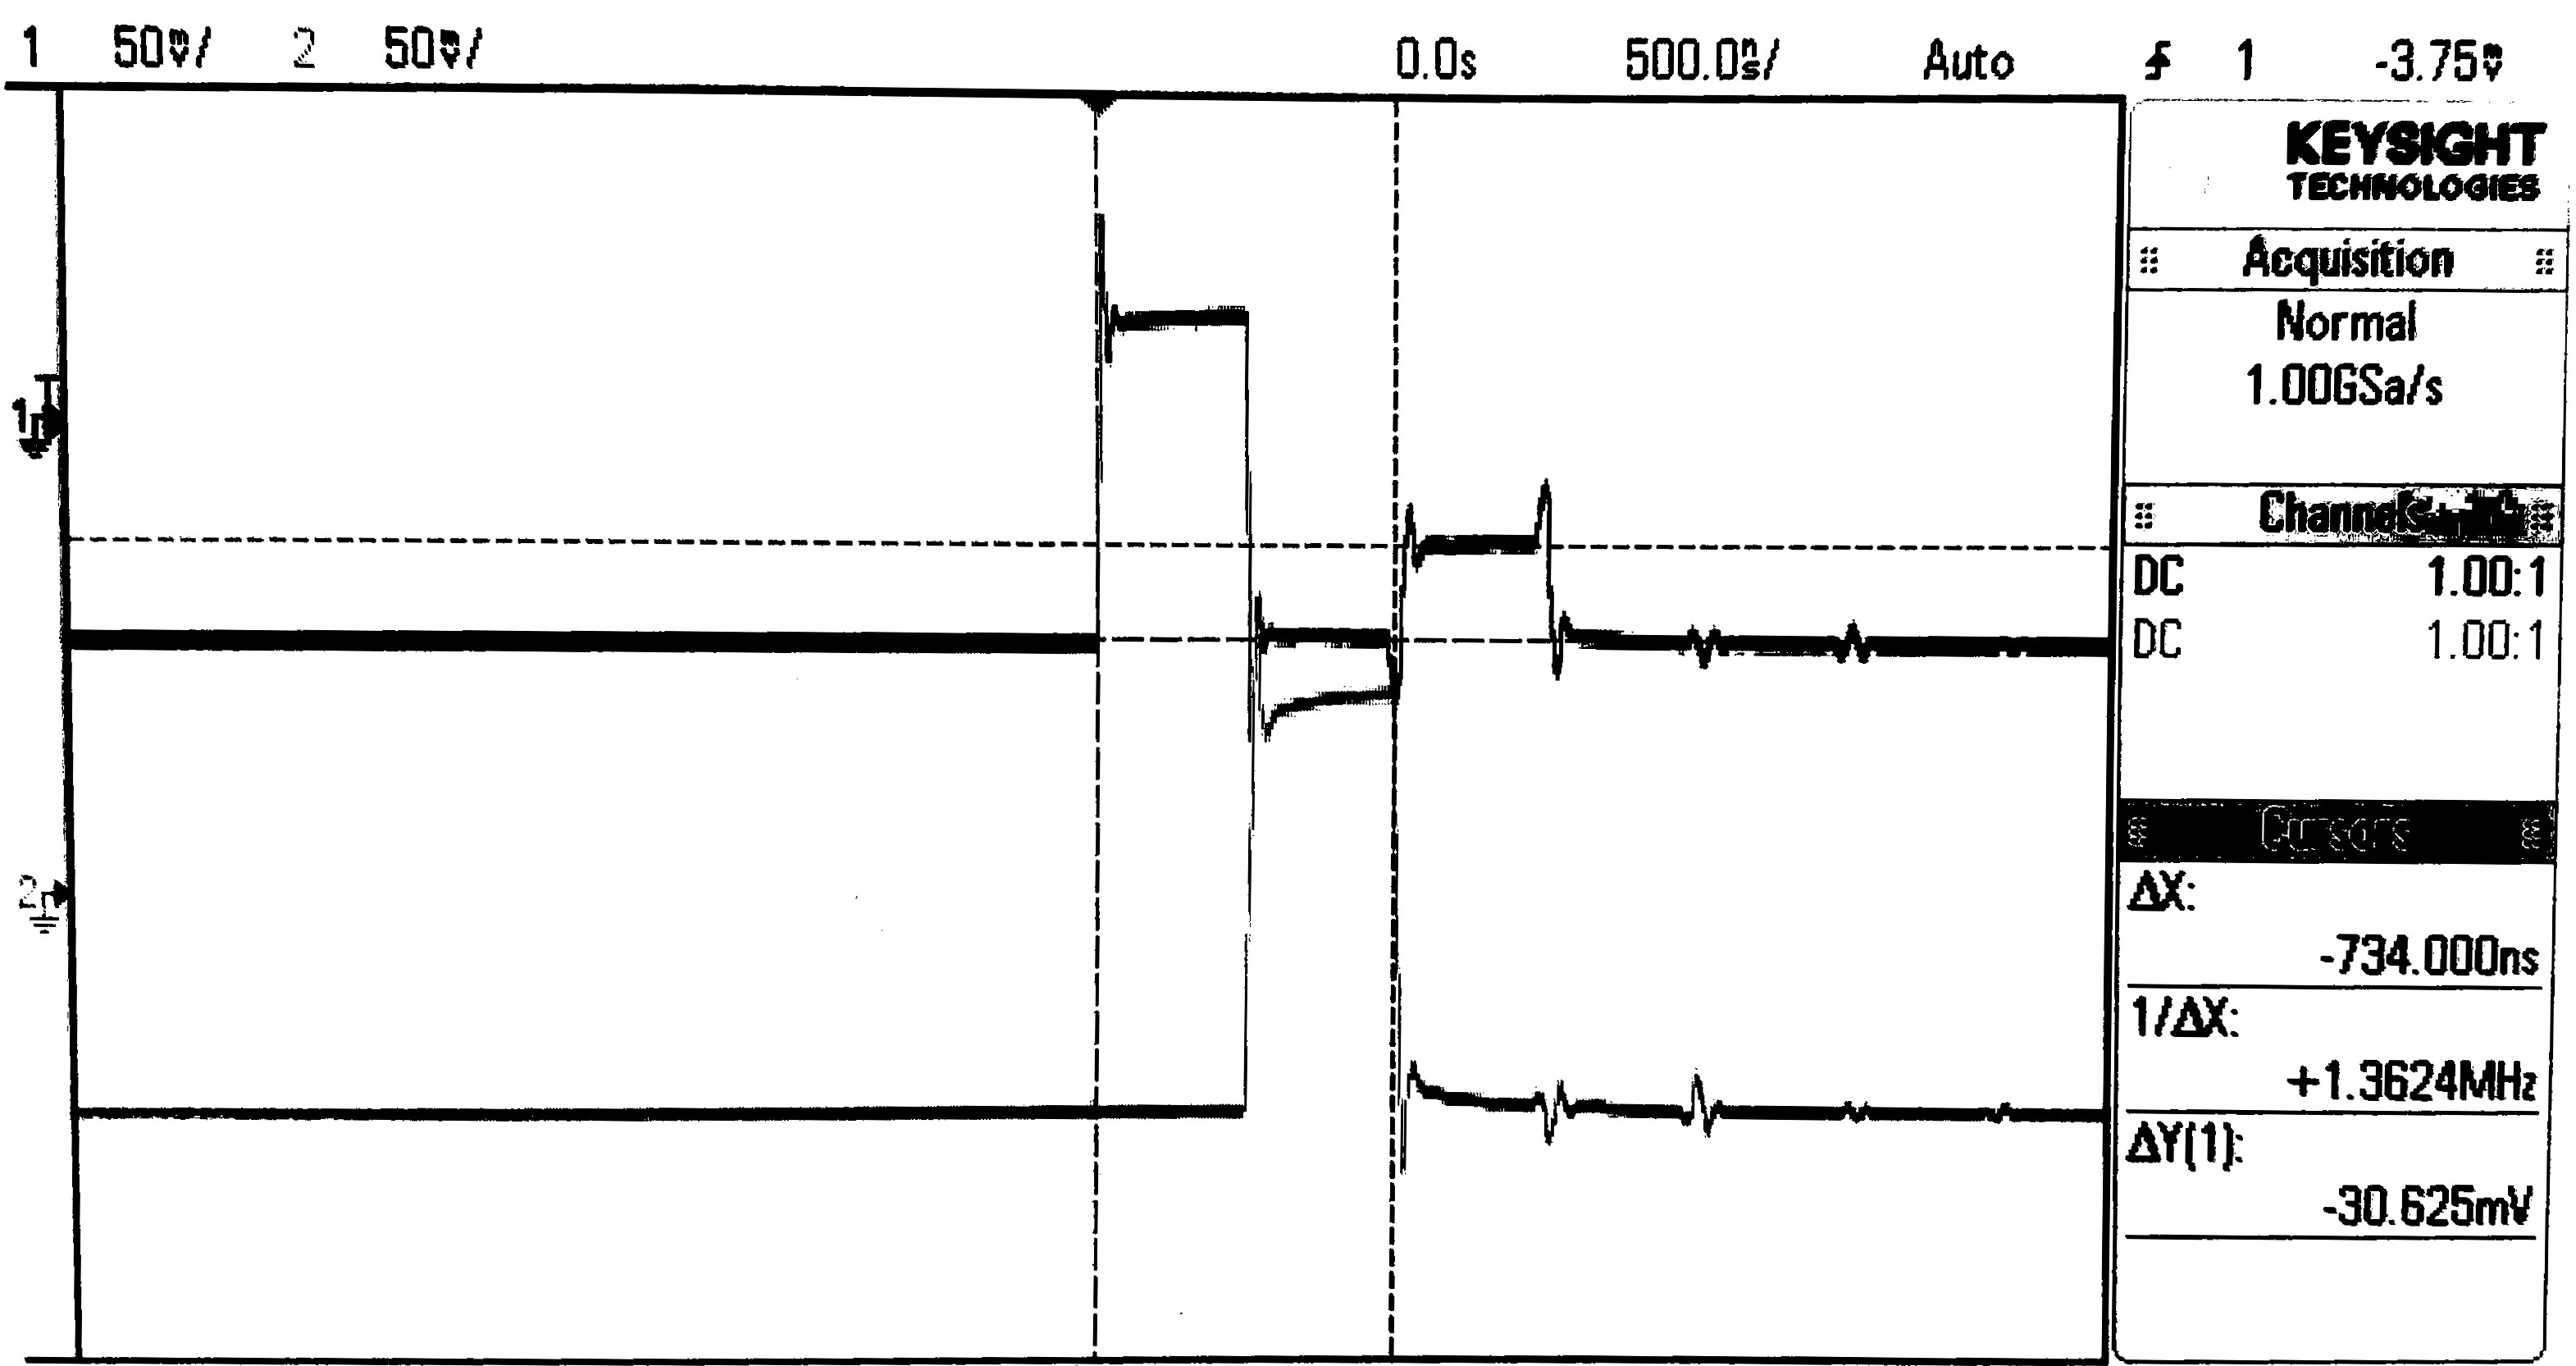
\includegraphics[width=\textwidth]{../photos/lab1/v_t_gamma_L_2.jpg}
%         \caption{$\tilde V_2 = \Gamma_L\tilde V^+ = \tilde V^- \approx 30\text{mV}$}
%     \end{subfigure}
%     \caption{$\tilde V$ measured at port C and port F for input signal with pulsewidth $\tau = T$\vspace{-0.5cm}}
%     \label{v_t_c_f}
% \end{figure}

% \begin{figure}[h]
%     \centering
%     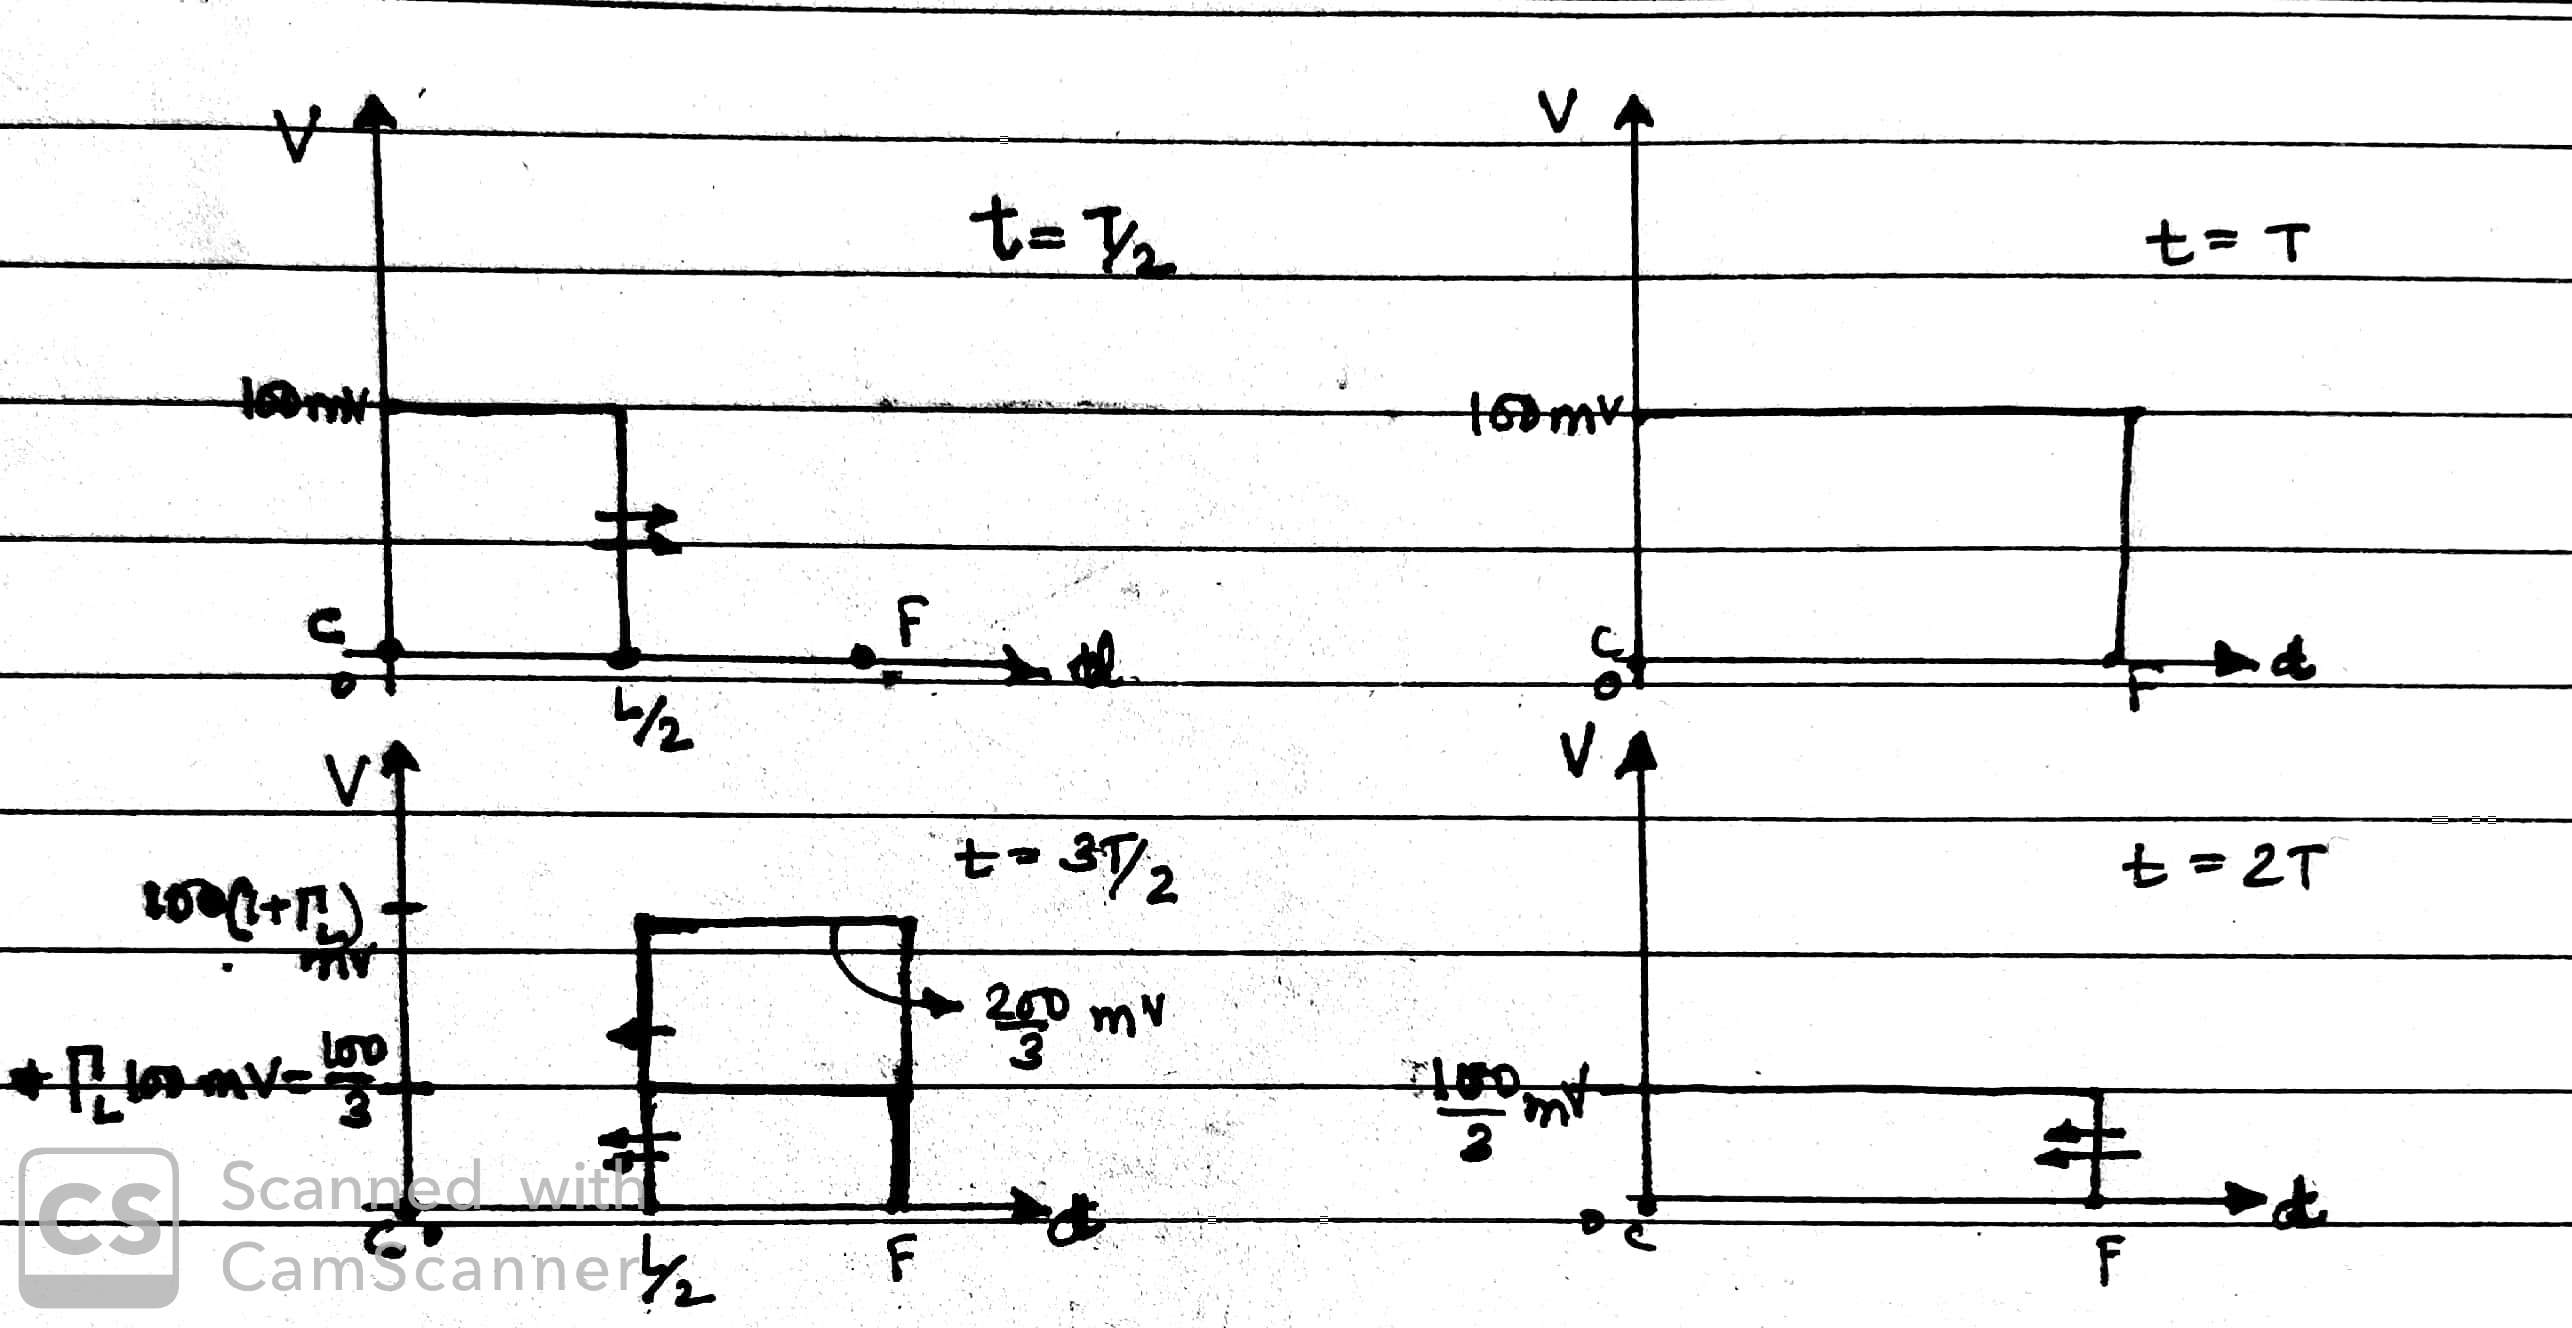
\includegraphics[width=0.45\textwidth]{../photos/lab1/v_d_gamma_L.jpg}
%     \caption{$V(d)$ plots at different time points\vspace{-0.5cm}}
%     \label{v_d_different_T}
% \end{figure}

% \section{Multiple Reflections}

% For mismatched generator side, $Z_g = 150\Omega$, as well as the load side, $Z_L = 20\Omega$, there will 
% be reflections on both ends of the transmission line. The observed waveforms can be found in Figure 9, with channel 1 (top) recording
% signals at port C and channel 2 (bottom) recording signals at port F.

% \begin{figure}[ht]
%     \centering
%     \begin{subfigure}[b]{0.45\textwidth}
%         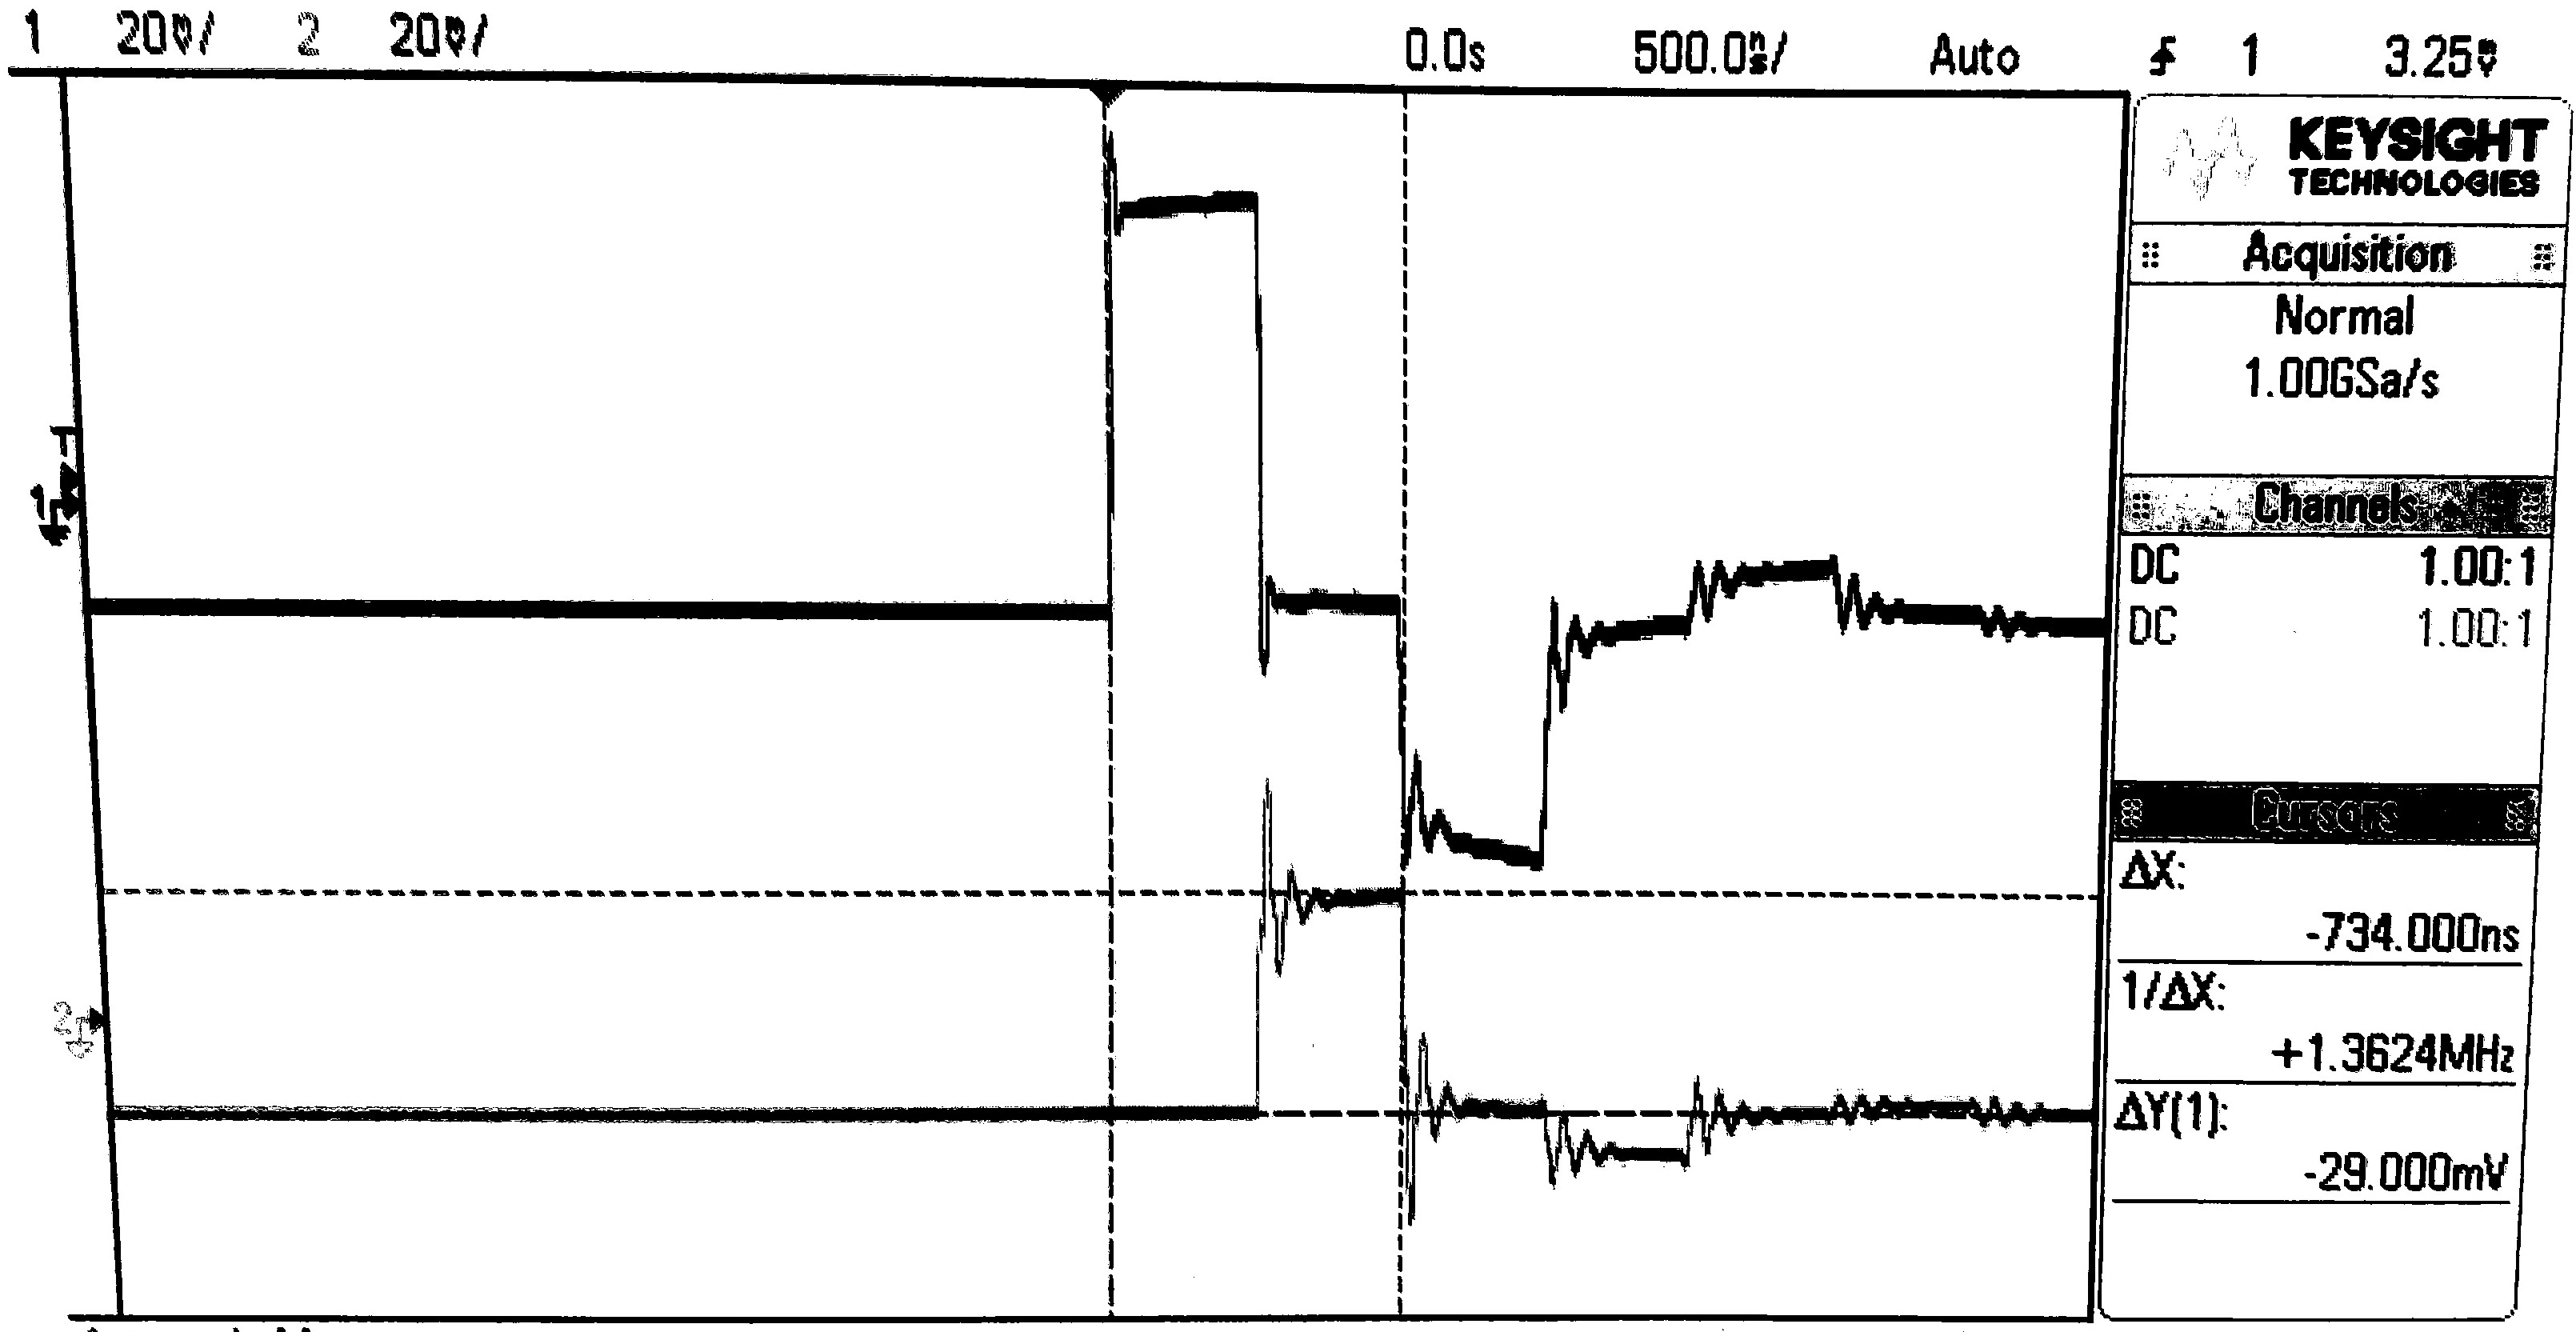
\includegraphics[width=\textwidth]{../photos/lab1/v_t_gamma_mult_1T.jpg}
%         \caption{$\tau = T$}
%     \end{subfigure}
%     \quad
%     \begin{subfigure}[b]{0.45\textwidth}
%         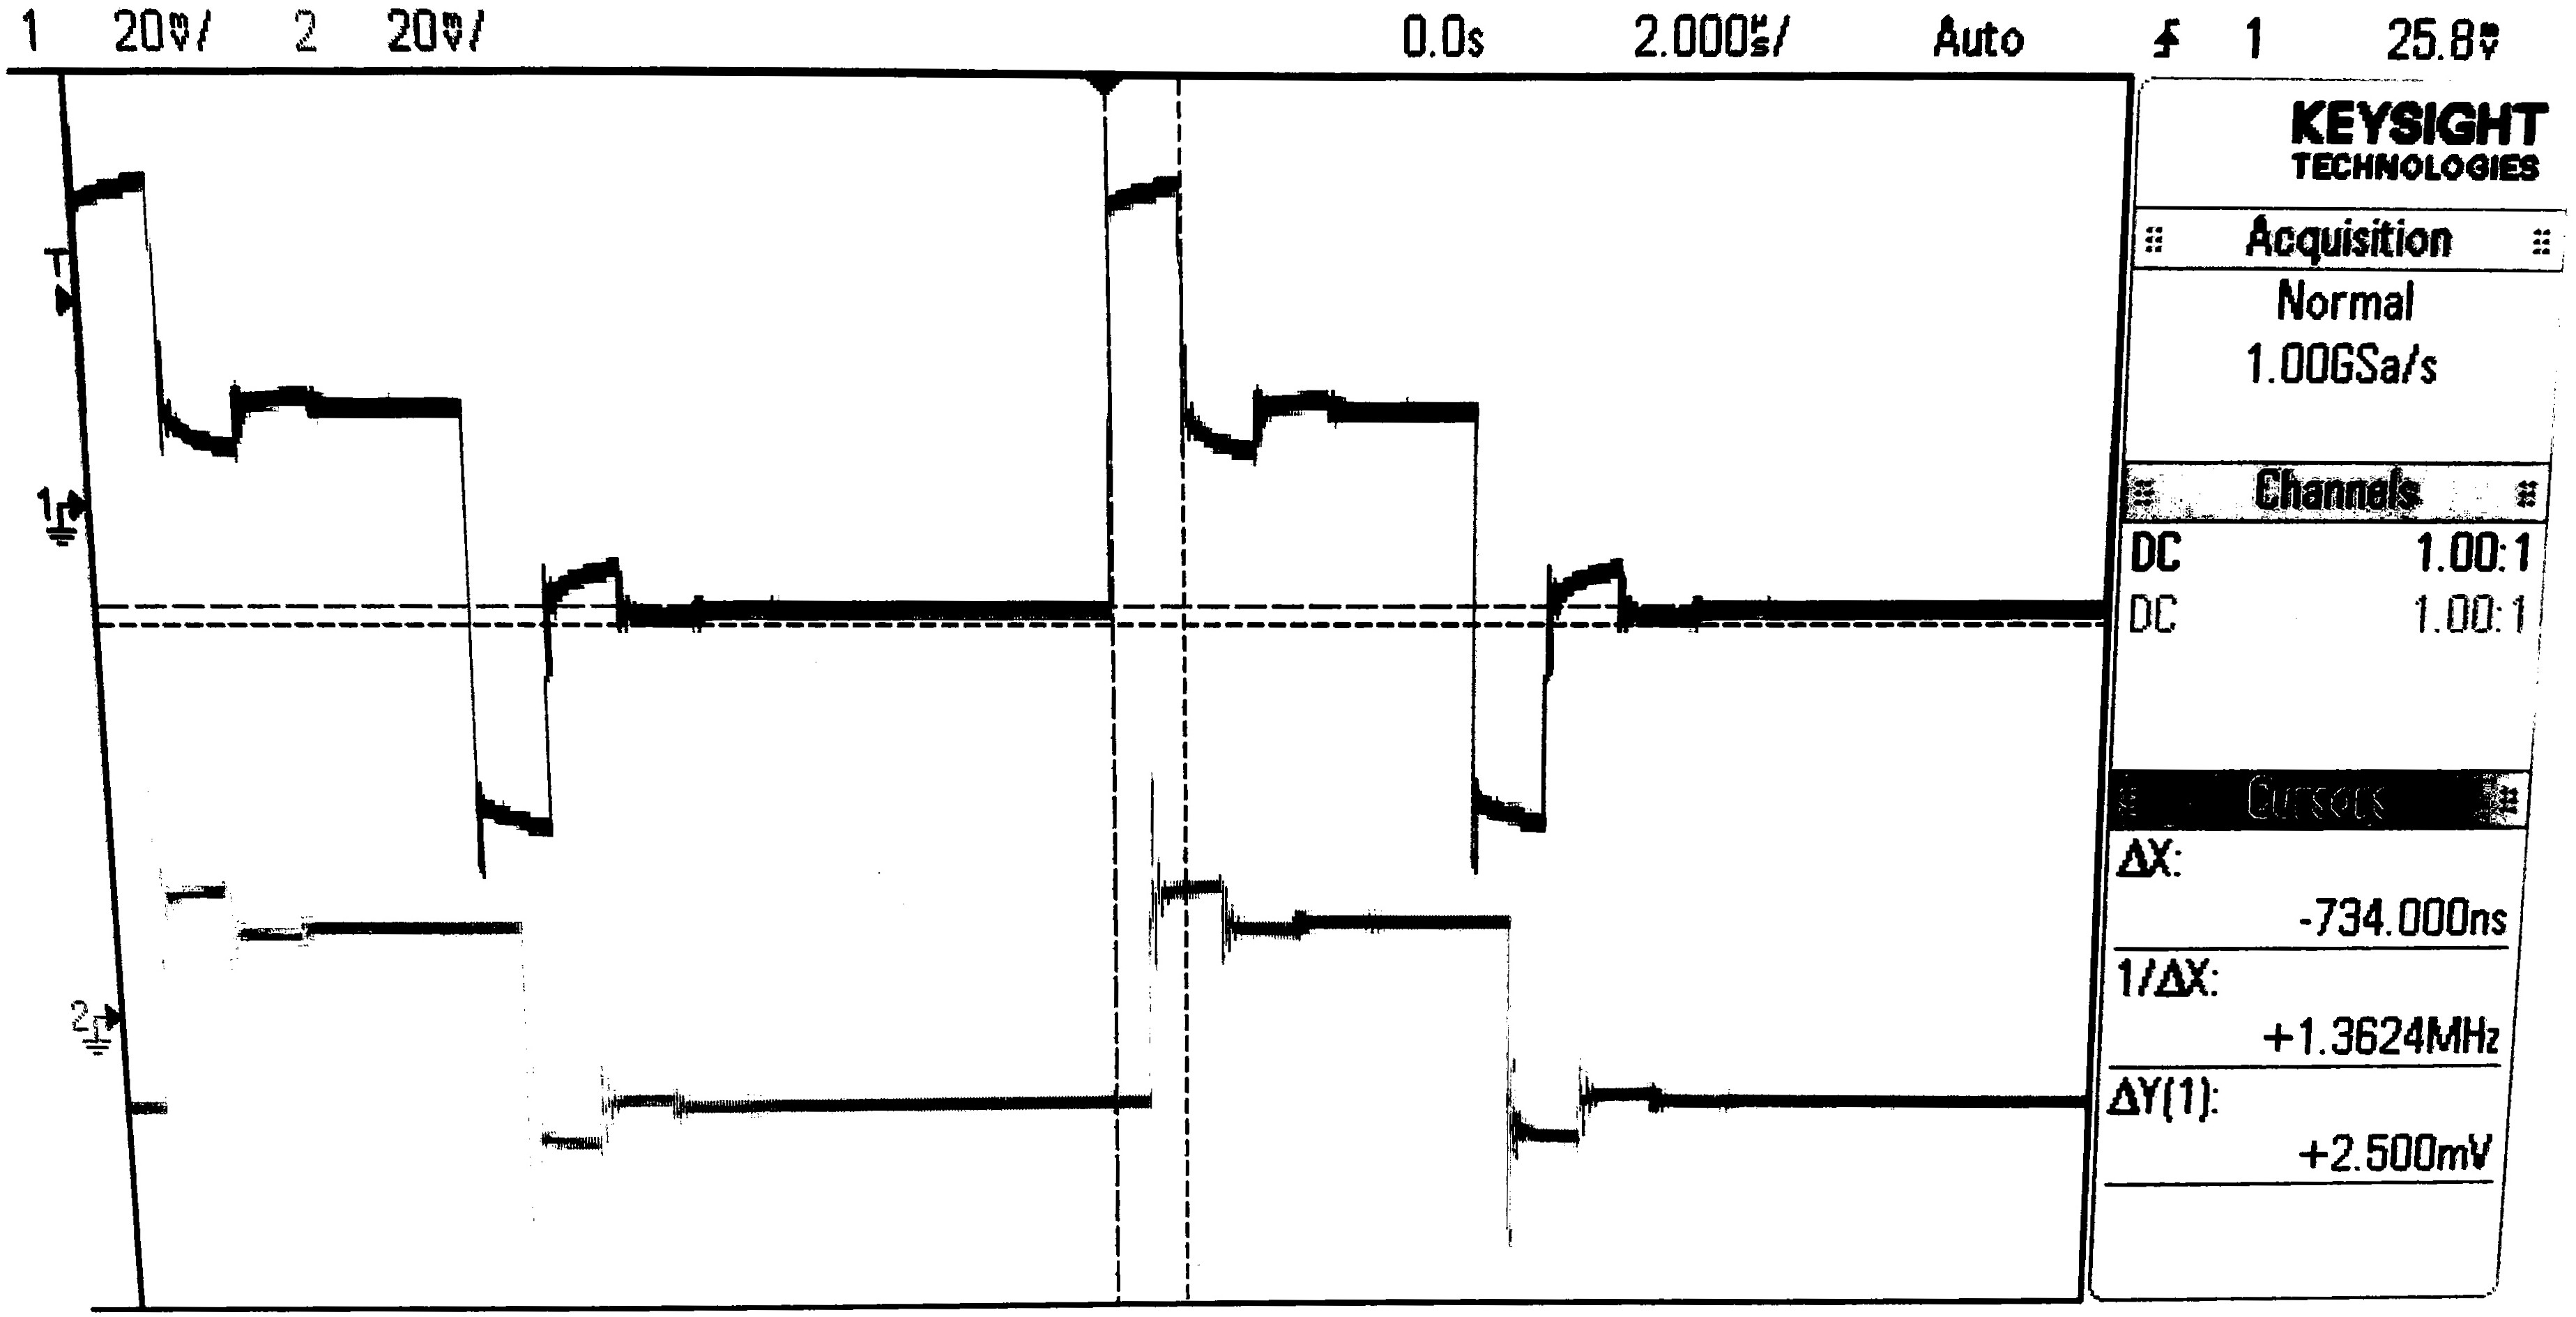
\includegraphics[width=\textwidth]{../photos/lab1/v_t_gamma_mult_10T.jpg}
%         \caption{$\tau = 10T$}
%     \end{subfigure}
%     \caption{Multiply reflected signals for input signal with different pulsewidths\vspace{-0.4cm}}
%     \label{v_t_ref_mult}
% \end{figure}

% At the generator end of the transmission line, $\Gamma_g = \frac{100 \Omega}{200 \Omega} = \frac{1}{2}$, and
% at the load end $\Gamma_L = \frac{-30 \Omega}{70 \Omega} = \frac{-3}{7}$. In Figure 9 (a), we measure
% $\tilde V^+ = \tilde V_1^+ = 51.5\text{mV}$ on channel 1 for $t \in (0, T)$, whereas on channel 2 for $t \in (T, 2T)$, we measure $\tilde V = \tilde V^+ + \tilde V^- = 29\text{mV}$.
% This implies that $\tilde V^- = \Gamma_L\tilde V^+ = 29 - 51.5\text{mV} = -22.5\text{mV}$. Therefore, the observed 
% $\Gamma_L = \frac{\tilde V^-}{\tilde V^+} = \frac{-22.5\text{mV}}{51.5\text{mV}} = -0.437 \approx \frac{-3}{7}$. Similarly, in Figure 9 (a), 
% we measure $\tilde V = \Gamma_L\tilde V_1^+ + \Gamma_g\Gamma_L\tilde V^+_1 = -32\text{mV}$ at port C (channel 1) for $t \in (2T, 3T)$.
% Here we use the previous measurement of $\Gamma_L = -0.437$, we measure $\Gamma_g = 0.42 \approx \frac{1}{2}$. Thus, both of our 
% measurements closely match the theoretical values for the reflection coefficients.

% \begin{figure}[ht]
%     \centering
%     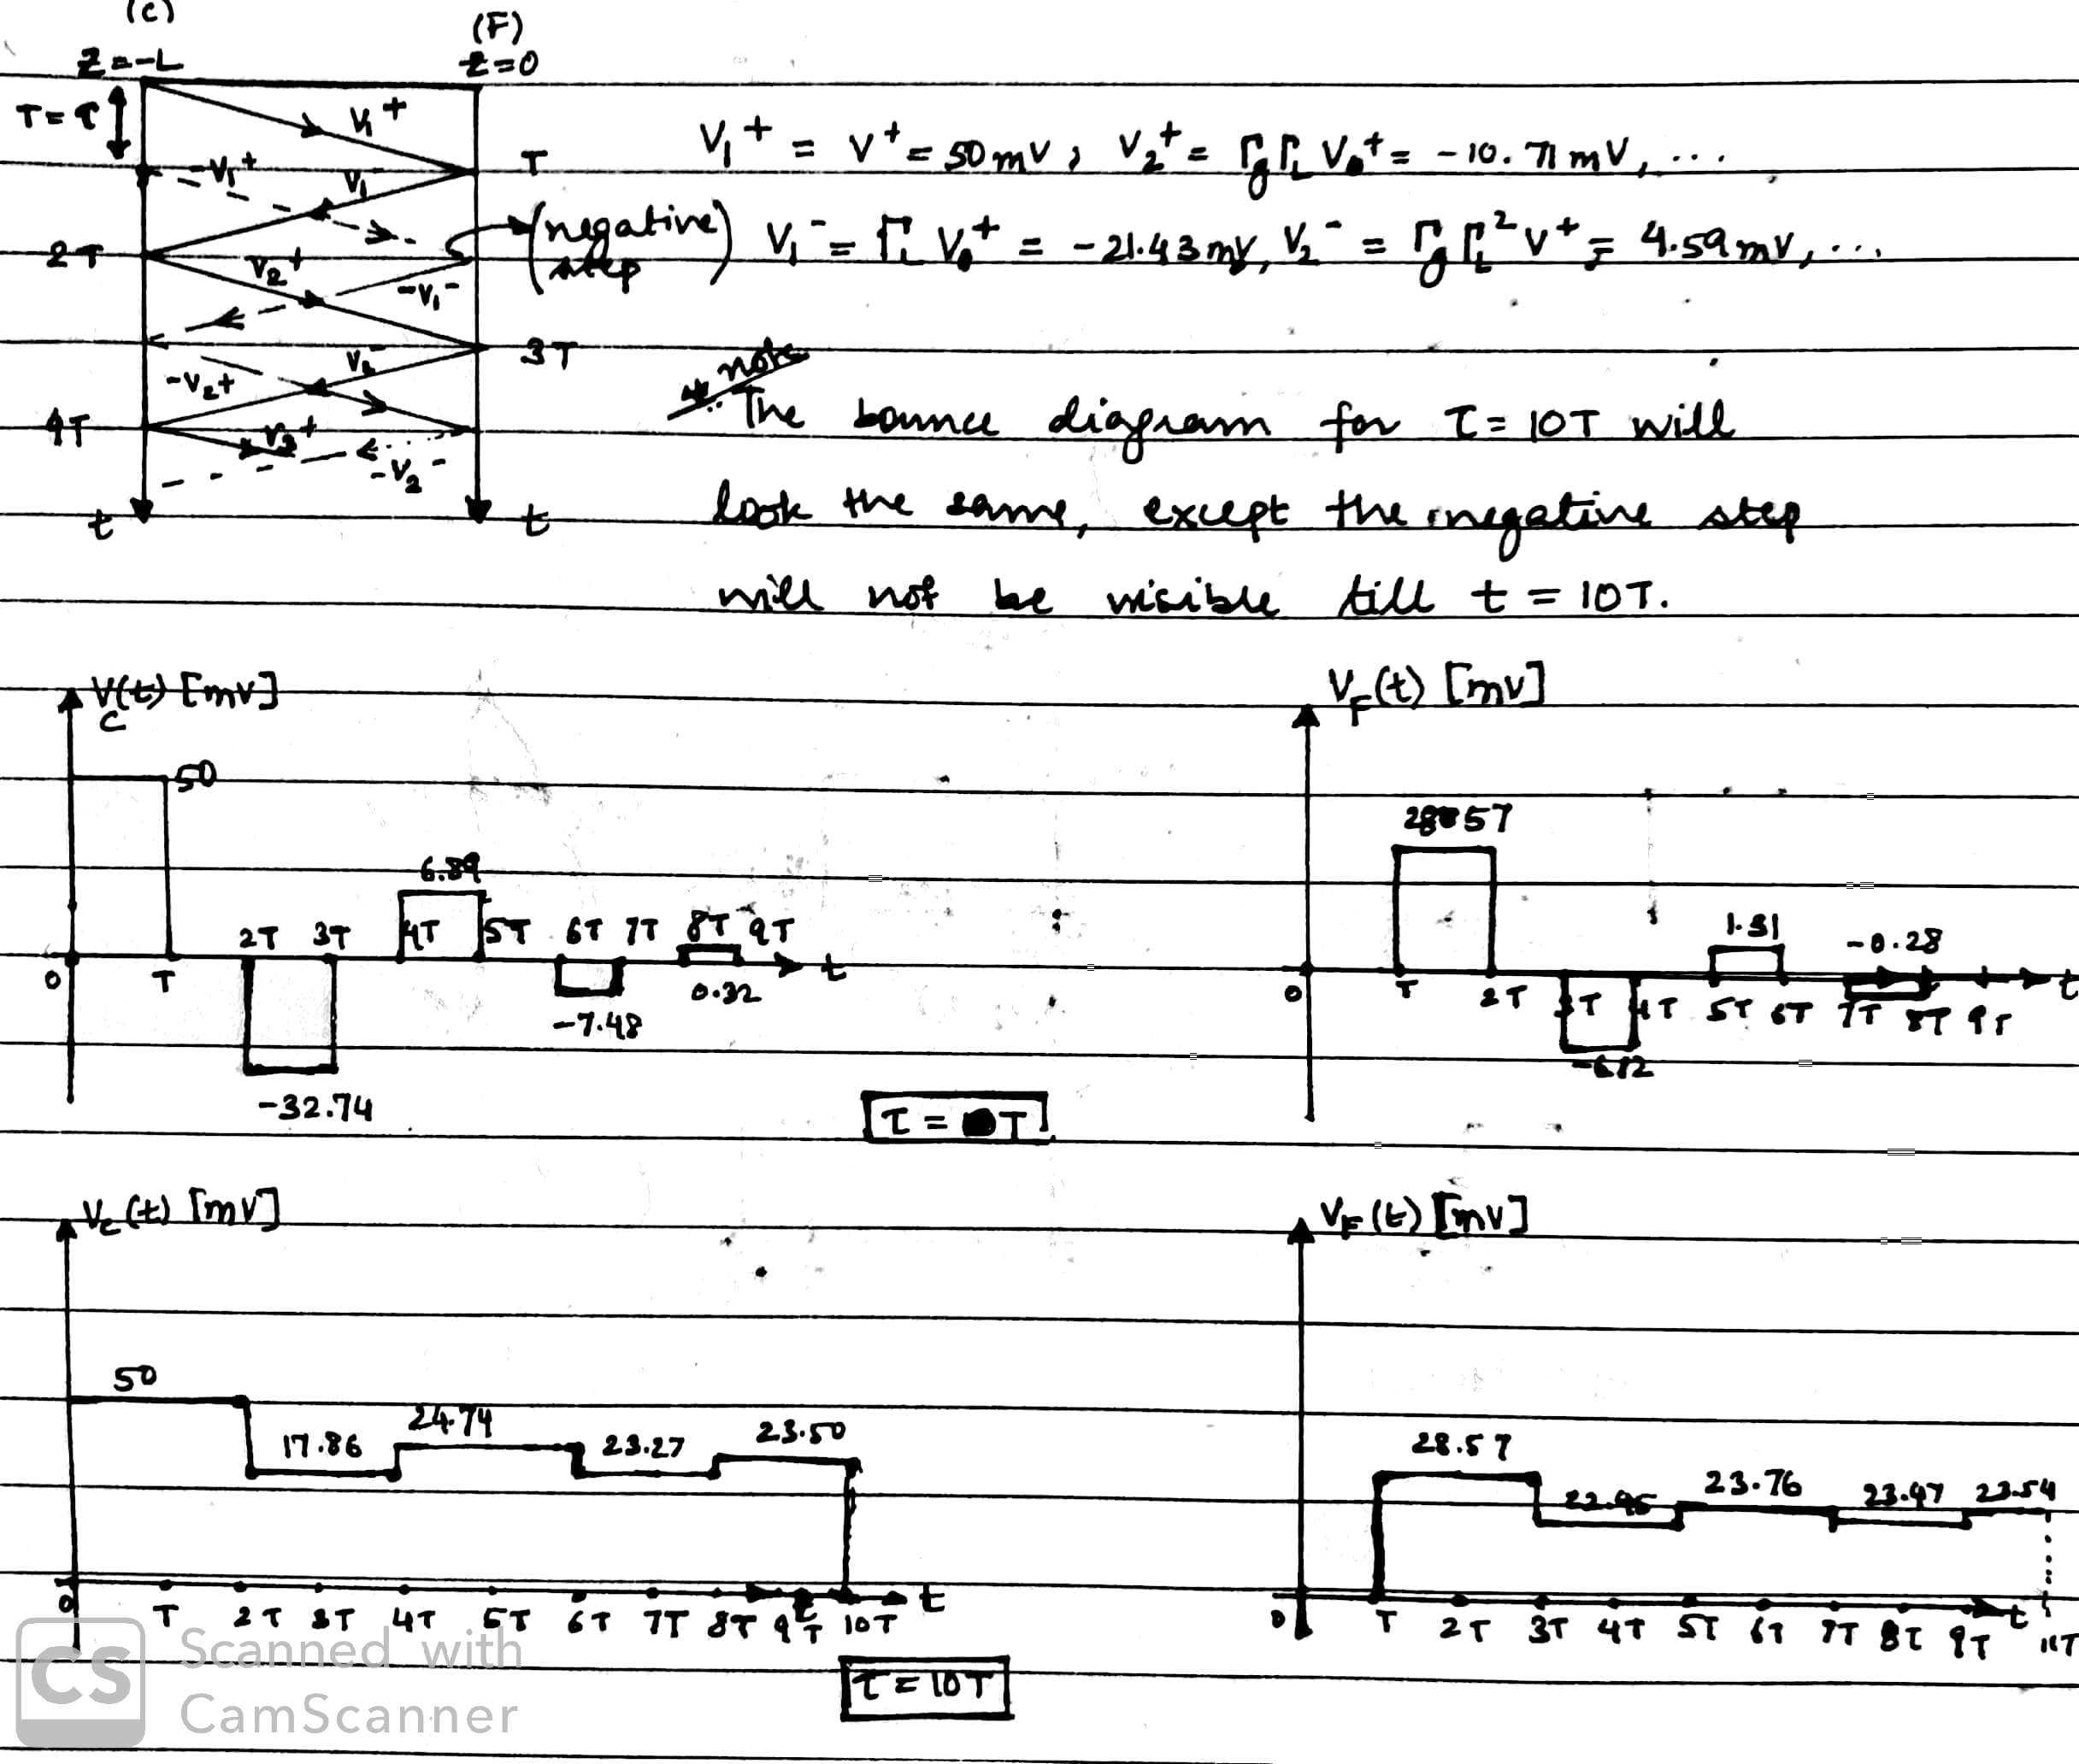
\includegraphics[width=0.7\textwidth]{../photos/lab1/v_t_bounce_mult_ref.jpg}
%     \caption{Theoretical bounce diagrams and $V(t)$ plots for $\tau = T$ and $\tau = 10T$\vspace{-0.5cm}}
%     \label{v_t_bounce_mult}
% \end{figure}

% Theoretical bounce diagrams and $V(t)$ plots for signals observed at ports C and F can be found in Figure 10. In Figures 9 and 10, 
% we observe such behavior of pulses because the input pulse creates a reflection at the load which comes back to the source; however,
% when the reflection reaches the source, it is also being reflected and, thus, the source and load in this setup 
% keep the pulse bouncing back and forth until it completely dies out beacuse of resistive losses along the transmission line.


% \section{Input Impedance and Transmission Line Length}

% While sweeping the input sinusoid frequency from 1MHz to 4MHz, we recorded the frequencies at 
% which $||\tilde V_\text{in}||$ achieved its minimum. These frequencies are listed in Table 2.
% \begin{table}[ht]
%     \[
%         \begin{array}{c|c}
%             f_\text{min} \textbf{ Shorted} &  f_\text{min} \textbf{ Capacitive} \\ \hline
%             1.4 & 1.6\\
%             2.8 & 3.0\\
%             4.0 & 4.2
%         \end{array}
%     \]
%     \caption{Corresponding $f_\text{min}$ for minimum $\tilde V_\text{in}$ for zero and capacitive loads in $\text{MHz}$\vspace{-0.5cm}}
% \end{table}

% \begin{figure}[ht] \centering
%     \begin{circuitikz} 
%         \draw
%         (0, 2) to [V, l_=$\tilde V_g$] (0, 0) -- (2, 0)
%         to [R, l_=${Z_{\text{in}}}$, -*] (2, 2)
%         to [R, l_=$Z_g$] (0, 2);

%         \draw (2, 2) -- (2.25, 2.25);
        
%         \draw 
%         (3.45, 2.4) 
%         node[]{$\displaystyle{\tilde V_{\text{in}} = \tilde V_g\frac{Z_{\text{in}}}{Z_{\text{in}} + Z_g}}$} 
%         (3.45, 2.4);
%     \end{circuitikz}
%     \caption{Voltage division over net input impedance, $Z_\text{in}$\vspace{-0.5cm}}
%     \label{volt_diag}
% \end{figure}

% To explain this effect for the short circuited (zero) load, we know that $\Gamma_L = -1 \implies \phi_\Gamma = \pi$ and the voltage along the transmission line is 
% $\tilde V(z) = \tilde V_0^+e^{-j\beta z}(1 + ||\Gamma_L|| e^{j2\beta z + j\phi_\Gamma})$. Thus, the voltage minimum occurs
% when $\phi_\Gamma + 2\beta z = (2k + 1)\pi, k \in \mathbb{Z}$. Since $\beta \propto \omega$, as we increase frequencies, there is a 
% change in $||\tilde V(z)||$. Also, since current $\tilde I = \frac{\tilde V_0}{Z_0}e^{-j\beta z}(1 - ||\Gamma||e^{j2\beta z + j\phi_\Gamma})$, there is a current maximum
% at voltage minimum, as when $||(1 + e^{j2\beta z + j\phi_\Gamma})||$ is minimum $||(1 - e^{j2\beta z + j\phi_\Gamma})||$ will be at its maximum.


% To explain voltage minimum for the capacitive load, we know that net input impedance of the load and transmission line at the source, $Z_in$, varies with frequency:
% \[
%     Z_{\text{in}} = Z(z)\big\rvert_{z=-L} = Z_0 \frac{1+\Gamma e^{j2\beta z}}{1-\Gamma e^{j2\beta z}}\bigg\rvert_{z=-L} = Z_0 \frac{Z_L + jZ_0\tan{\beta L}}{Z_0 + jZ_L\tan{\beta L}}
% \]

% Thus, at certain frequencies, when $Z_\text{in}$ is minimum, $||\tilde V_\text{in}||$ will also be minimum. To find frequencies at which this minimum will occur,
% we know that now $\Gamma = \frac{jX_c(\omega) - Z_0}{jX_c(\omega) + Z_0} = ||\Gamma||e^{j\phi_\Gamma}$. Here, we note that for a pure
% capacitive load $||\Gamma|| = 1$ and phase is a function of frequency, $\phi_\Gamma(\omega) = 2\arctan(\frac{10^8j}{50\omega})$ for $C = 0.01\mu F$, as opposed to the short circuited load where $\phi_\Gamma = \pi$.
% Thus, the voltage minimums will occur at $2\beta z + \phi_\Gamma(\omega) = (2k+1)\pi, k \in \mathbb{Z}$, where $f_\text{min}$ will be skewed beacuse of the frequency-depedance of reflection coefficient's phase.

\section{Notes}

All images taken during the lab were post-processed in a batch using a custom script
that bit-wise inverts the pixels and binarizes the resulting image based on a custom threshold.
No adjustments or modifications were made to the readings, for which the oscilloscope's measurements
are also shown alongside the waveforms. All scripts and related work can be found at 
\href{https://github.com/pranshumalik14/ece320-labs}{\texttt{github.com/pranshumalik14/ece320-labs}}.

\end{document}